\documentclass[mathserif,10pt]{beamer}
% insert "handout" into the options argument of the documentclass
\usetheme{CambridgeUS}
\usecolortheme{beaver}
\usepackage{amsmath}
\usepackage{graphicx}
\usepackage{epstopdf}
\usepackage{xcolor}
%\usepackage{epstopdf}
%\usepackage{pdfpages}
\usepackage{media9}
%\usepackage{mdframed}
\DeclareGraphicsRule{.tif}{png}{.png}{`convert #1 `dirname #1`/`basename #1 .tif`.png}
\usepackage{hyperref}
%\usepackage[T1]{fontenc}

\setbeamertemplate{navigation symbols}{}
\setbeamertemplate{items}[triangle]
\setbeamertemplate{section in toc}[ball unnumbered]
%\definecolor{my red}{fg={\usebeamercolor[fg]{palette primary}}}
%\setbeamercolor{button}{bg={\usebeamercolor[fg]{alerted text} red}, fg=white}

%\addtobeamertemplate{footline}{\insertframenumber / \inserttotalframenumber}

% To show TOC with current section highlighted at the 
% beginning of each section
\AtBeginSection[]
{
  \begin{frame}
  \frametitle{}
  \tableofcontents[currentsection]
  \end{frame}
}

% To turn off section review slide for a section
% { 
%  \AtBeginSection[]{}
%    \section{Example}
%    \frame{Example}
% }


\title[Gravitational Collapse in AdS]{Gravitational Collapse in Anti-de Sitter Space}
\author[Brad Cownden]{Brad Cownden \\ PhD Thesis Defence}
\date[June --, 2020 UM]{June --, 2020 \\ University of Manitoba}


\newcommand{\bi}{\begin{itemize}}
\newcommand{\ei}{\end{itemize}}
\newcommand{\its}{\item}
\newcommand{\be}{\begin{align*}}
\newcommand{\ee}{\end{align*}}
\newcommand{\td}{\tilde}
\newcommand{\wtn}{\widetilde{\nabla}}
\newcommand{\del}{\nabla}
\newcommand{\h}{\hat}
\newcommand{\p}{\partial}
\newcommand{\til}{\tilde}
\newcommand{\w}{\wedge}
\newcommand{\sh}{\hat\star}
\newcommand{\st}{\tilde\star}
\newcommand{\mc}{\mathcal}
\newcommand{\sla}{\slashed}
\newcommand{\scr}{\scriptsize}
\newcommand{\jm}{j_{max}}

\begin{document}

%%%%%%%%%%%%%%%%%%%%%%%%%%%%%%%%%%%%%%%%%%%%%%
%%%%%%%%%%%%%%%%%%%%%%%%%%%%%%%%%%%%%%%%%%%%%%

\frame
{
   \titlepage
   \begin{center}
   
\includegraphics[scale=0.25]{newlogos}
   \end{center}
}

\frame
{
  \frametitle{}
  \tableofcontents
}

%%%%%%%%%%%%%%%%%%%%%%%%%%%%%%%%%%%%%%%%%%%%%%
%%%%%%%%%%%%%%%%%%%%%%%%%%%%%%%%%%%%%%%%%%%%%%
{
  \AtBeginSection[]{}
\section{Gravitational Collapse}
\frame
{
  \frametitle{Gravitational Collapse}
  \bi
  \its Numerical studies of gravitational collapse in Minkowski spacetime: horizon size = power law\footnotemark , mass gap
  \its AdS/CFT $\to$ thermal quench in gauge theory $\Leftrightarrow$ formation of black hole in gravitational theory
  \its Massless scalar fields in AdS: unstable against generic initial data, no mass gap\footnotemark\ $\to$ c.f. Minkowski
  \its Stability for specific initial data below critical energy
  \its Perturbative theory for stable/nearly-stable solutions
  \its {\bf Nonlinear theory:} continue with exploration of phase space\footnotemark
  \its {\bf Perturbative theory:} effects of truncation, space of solutions, evolution of nearly-stable solutions
  \ei	
  
  \footnotetext[1]{{\scr Choptuik PRL70 9 (1993)}} 
  \footnotetext[2]{{\scr Bizo\'n \& Rostworowski [1104.3702]}}
  \footnotetext[3]{{\scr Deppe \& Frey [1508.02709]}}
}
}

\frame
{
  \frametitle{Outline}
  \bi
  \its Manuscript thesis
  \ei
}

%%%%%%%%%%%%%%%%%%%%%%%%%%%%%%%%%%%%%%%%%%%%%%
%%%%%%%%%%%%%%%%%%%%%%%%%%%%%%%%%%%%%%%%%%%%%%

\section{Massive Scalars in AdS$_5$ [arXiv:1711.00454]}
\subsection{Phase Diagram \& Islands of Stability}
\frame
{
  \frametitle{Phase Diagram \& Islands of Stability}
  \begin{columns}
  \column{0.6\textwidth}
    \begin{itemize}
    \its Classical gravity in AdS$_{d+1}$ $\Leftrightarrow$ CFT in $d$-dimensions\footnotemark
    \its Scalar field in the bulk $\Leftrightarrow$ expectation value of operator in the boundary
    \its Heating vacuum state
    \its \alert{Black hole in AdS $\Leftrightarrow$ CFT in thermal equilibrium}
    \its Stability against collapse $\Leftrightarrow$ no thermalization
  \end{itemize}
  \column{0.4\textwidth}
    \begin{overlayarea}{\textwidth}{3cm}
    \begin{figure}
    \centering
    \only<1>{\hspace{-0.15in} 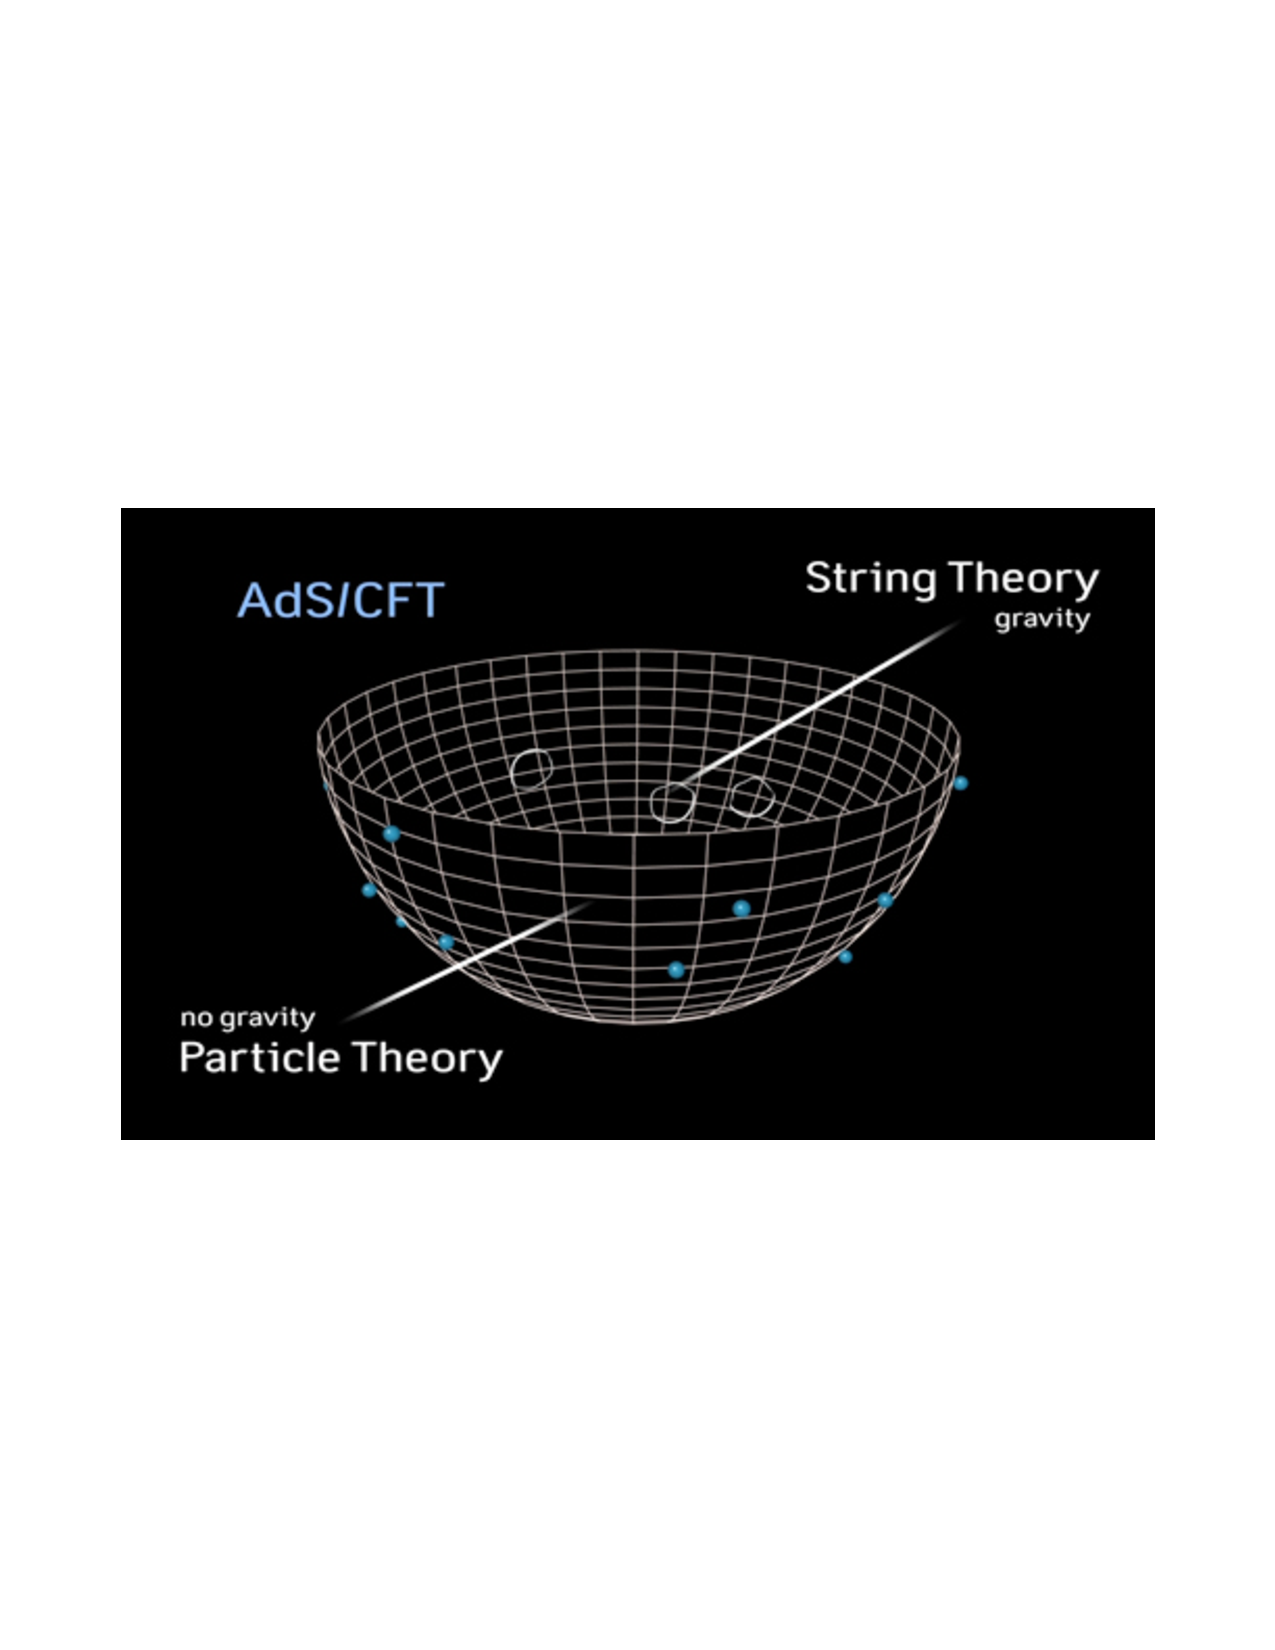
\includegraphics[scale=0.28]{adscft} \\ {\scr Learner.org}}
    \end{figure}
    \end{overlayarea}
  \end{columns}
  
  \footnotetext[4]{{\scr Maldecena [hep-th/9711200]}}
}

\frame % NB. Run in Presentation program to get proper playback
{
  \frametitle{Scalar Fields in Anti-de Sitter Spacetime}
  \bi
  \its Massless scalars: reflected off the boundary \href{run:./Massless_multi_bounce.mp4}{\beamerbutton{multiple times $\triangleright$}}, or \href{run:./masslessnobounce.mp4}{\beamerbutton{collapse immediately  $\triangleright$}}
    \its Massive scalars: can be gravitationally \href{run:./massive_long.mp4}{\beamerbutton{refocused  $\triangleright$}}, or also \href{run:./massive_short.mp4}{\beamerbutton{collapse immediately  $\triangleright$}}
    \its<2->{Classify as stable or unstable}
  \ei

  \uncover<2->{
    \begin{columns}
    \column{0.5\textwidth}
      \begin{figure}
      \centering
      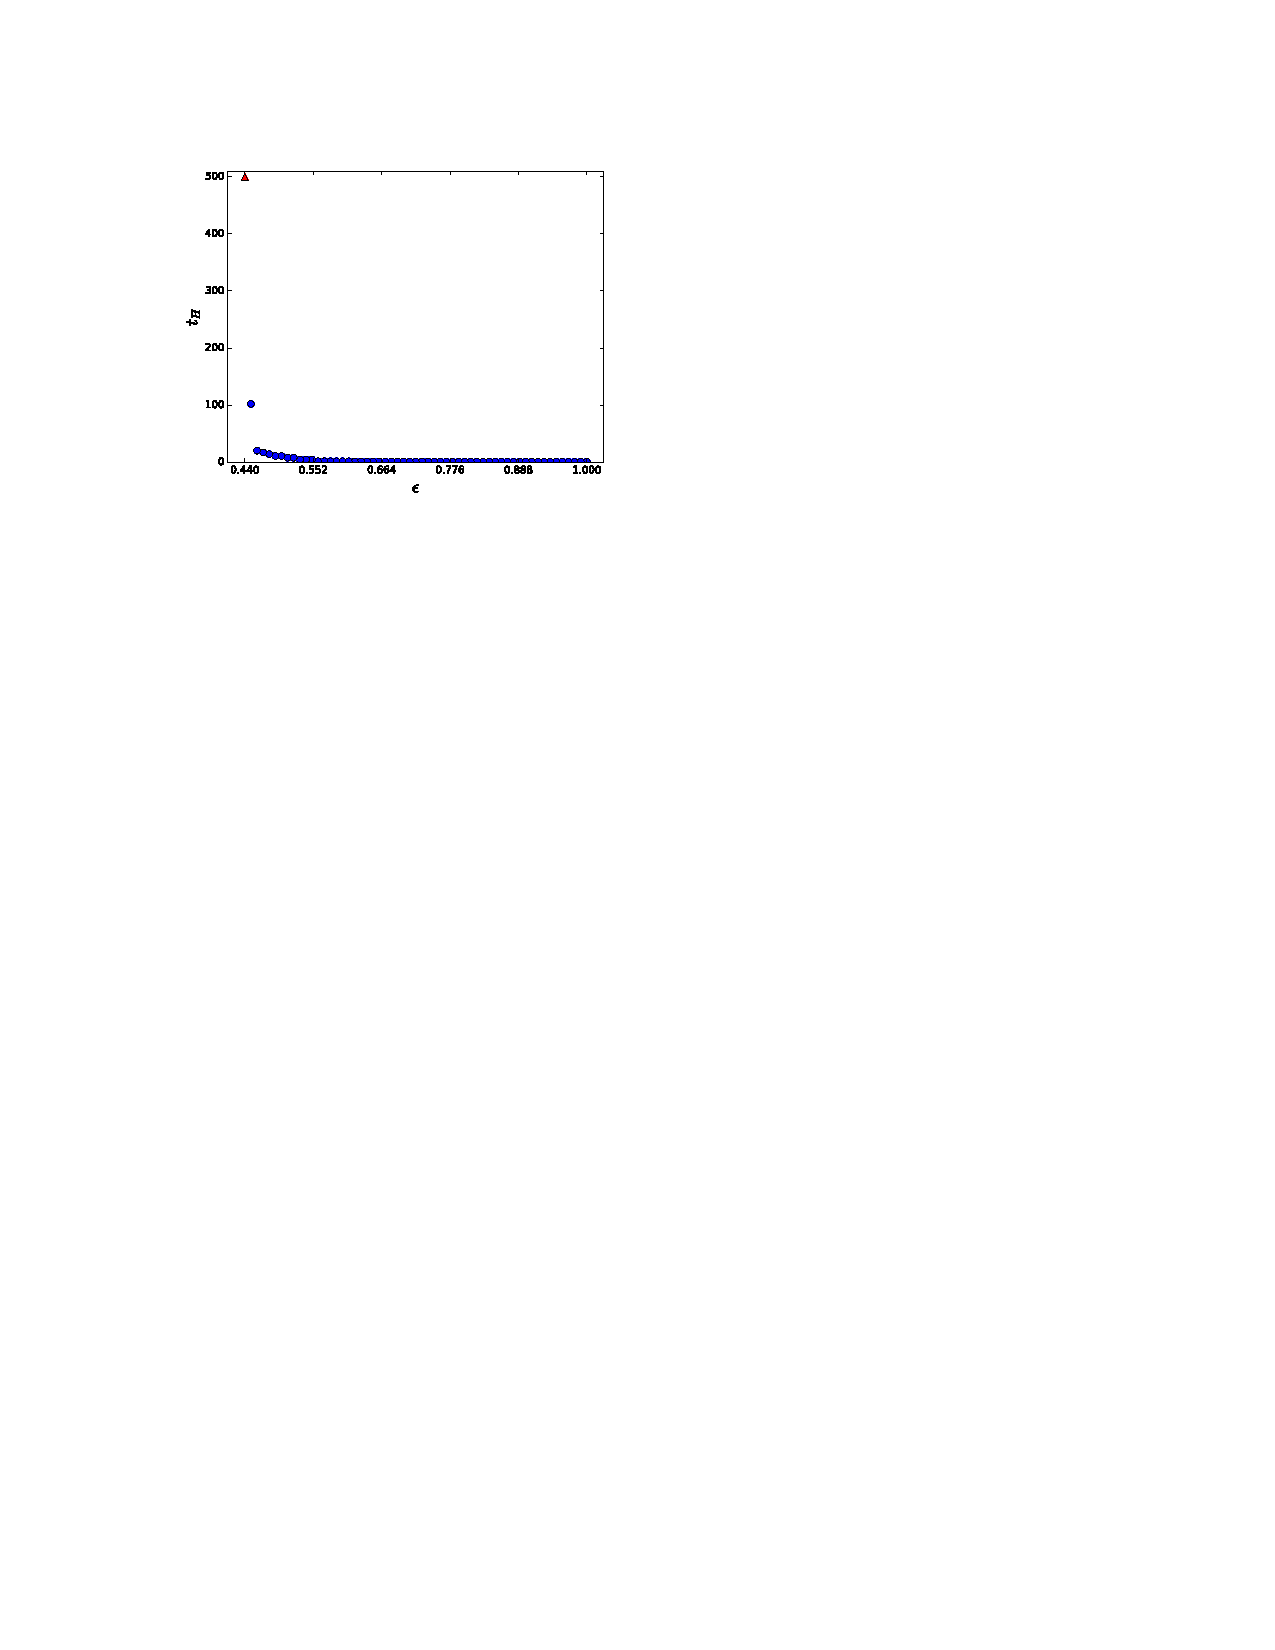
\includegraphics[scale=0.75]{m0w15} \\ $\mu = 0, \sigma = 1.5$
      \end{figure}
    \column{0.5\textwidth}
      \begin{figure}
      \centering
      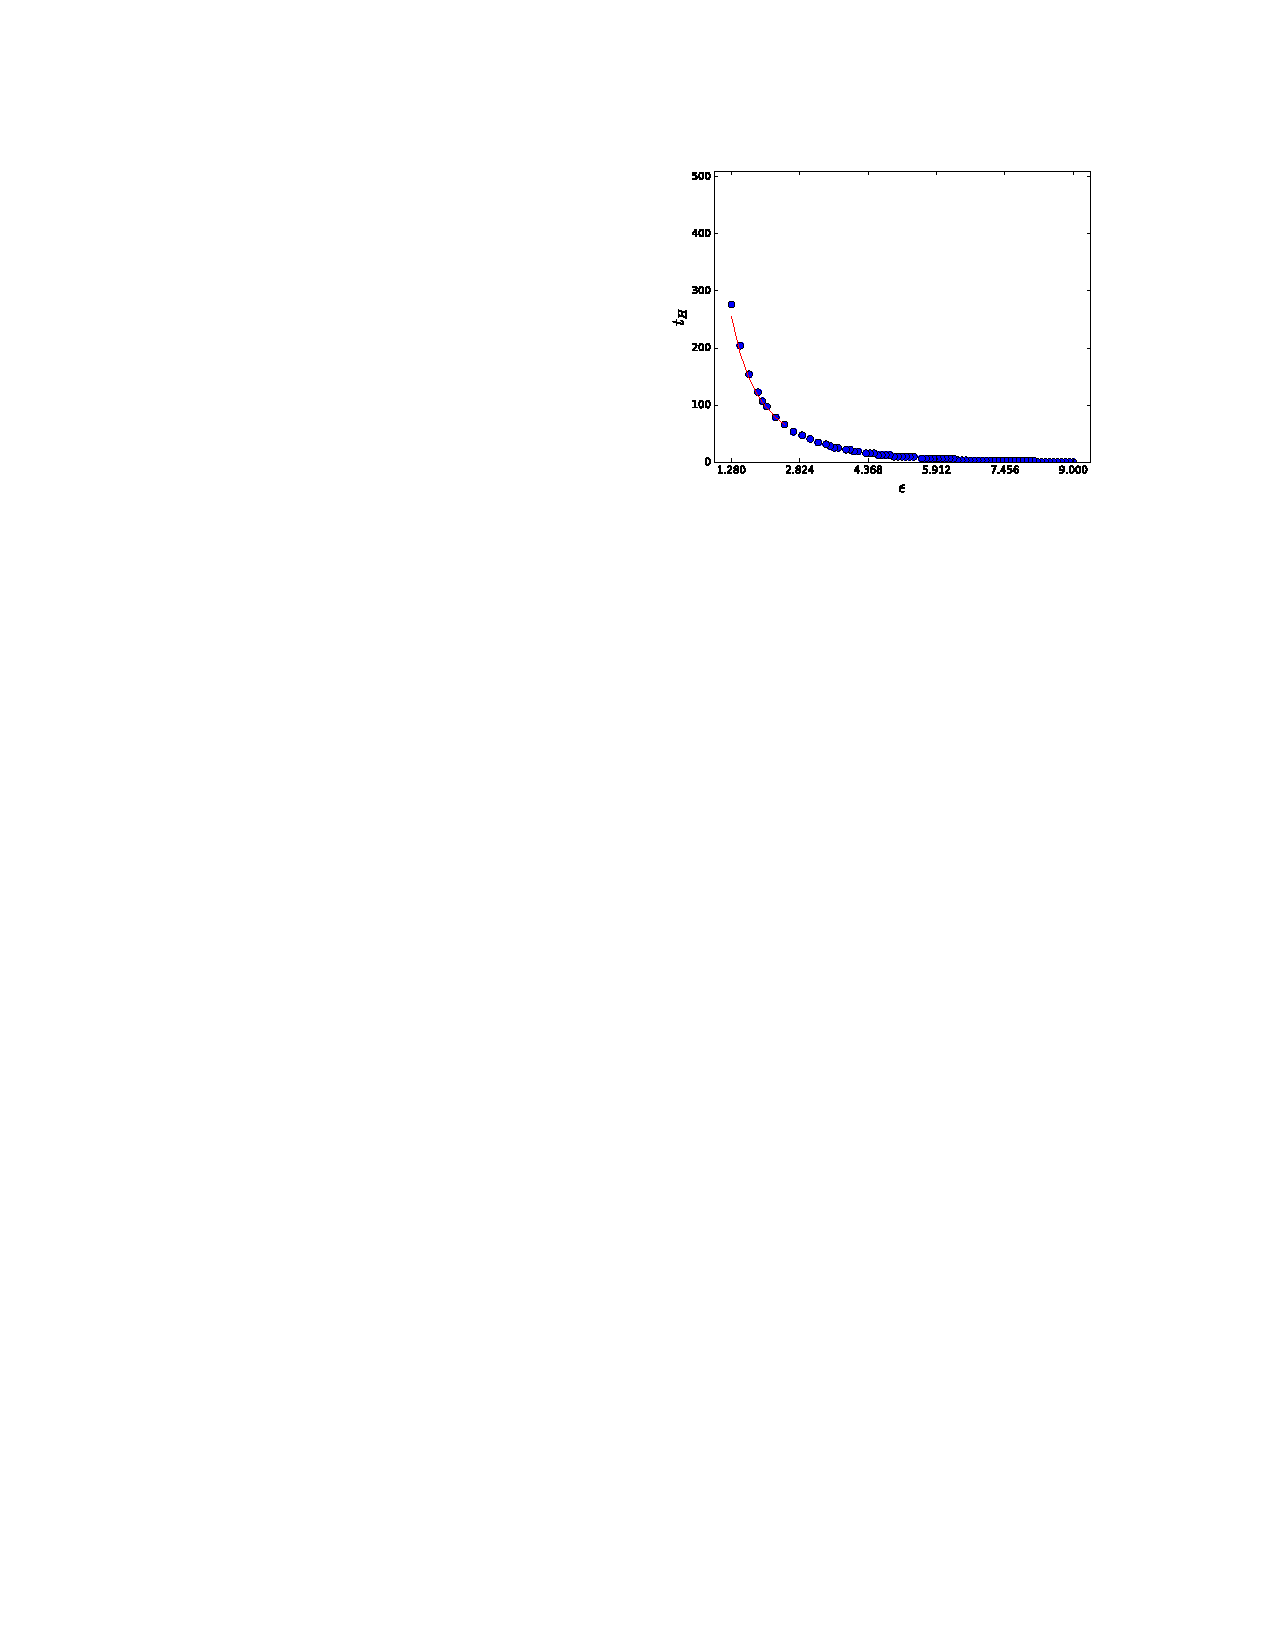
\includegraphics[scale=0.75]{m0w025} \\ $\mu = 0, \sigma = 0.25$
      \end{figure}
    \end{columns}
  }
}

%%%%%%%%%%%%%%%%%%%%%%%%%%%%%%%%%%%%%%%%%%%%%%

\subsection{Classifying Phases}
\frame
{
  \frametitle{Classifying Phases}
  \vspace{-0.7in}
  \bi
  \its Minimally-coupled scalar field in AdS$_5$ (dual to 4D CFT)
  \its Spherical symmetry, Schwarzschild-like coordinates $\to$ \alert<1>{$A(t,x)$}, \alert<1>{$\delta(t,x)$}
  \uncover<2->{\its Einstein + Klein-Gordon $\Rightarrow$ constraint equations}
  \uncover<2->{\its Interior gauge $\delta(t,x=0) = 0$, mass conservation at $x = \pi/2$, $\phi(t=0,x) = 0$}
  \uncover<2->{\its Canonical momentum $\Pi(t,x) = e^{\delta} A^{-1}  \p_t \phi$, define $\Phi(t,x) \equiv \p_x \phi$}
  \uncover<2->{\its Horizon formation when $A(t_H, x_H) \ll 1$}
  \ei

  \vspace{-0.2in}
  \begin{overlayarea}{\textwidth}{0.1cm}
    \begin{align*}
    \only<1>{
     ds^2 &= \frac{\ell^2}{\cos^2 (x/\ell)} \left( - \alert<1>{Ae^{-2\delta}} dt^2 + \alert<1>{A^{-1}} dx^2 + \sin^2 (x/\ell) d\Omega^{d-1} \right)
     }
     \only<2>{
     		\p_x \delta &= - \left( \Pi^2 + \Phi^2) \sin(x) \cos(x) \right) \\
     		\p_x M &= \frac{\tan^{d-1}(x)}{2} \left( A (\Pi^2 + \Phi^2) + \frac{\alert{\mu^2} \phi^2}{\cos^2(x)} \right) \\
		A &= 1 - \frac{2 M \sin^2(x)}{(d-1) \tan^d (x)} \\
    		\Pi(t=0, x) &= \epsilon \exp \left( - \frac{\tan^2(x)}{\alert{\sigma^2}} \right) \qquad \text{Phase space:} \: \alert{\mu, \; \sigma}
    }
    \end{align*}
  \end{overlayarea}
  \vfill

}

%%%%%%%%%%%%%%%%%%%%%%%%%%%%%%%%%%%%%%%%%%%%%%

\subsection{Spectra}
\frame
{
  \frametitle{Spectra}
  \bi
  \its
  \ei
}

%%%%%%%%%%%%%%%%%%%%%%%%%%%%%%%%%%%%%%%%%%%%%%
%%%%%%%%%%%%%%%%%%%%%%%%%%%%%%%%%%%%%%%%%%%%%%


\frame
{
  \frametitle{Phase Diagram}
  \bi
  \its<2->{{\color{orange} Unstable}\uncover<3->{, {\color[rgb]{.34,.69,0.29} metastable}, }\uncover<4->{{\color{red} irregular}, }\uncover<5->{and {\color{blue} stable} initial data}}
  \ei 
  \begin{figure}
  \centering
  \only<1>{
  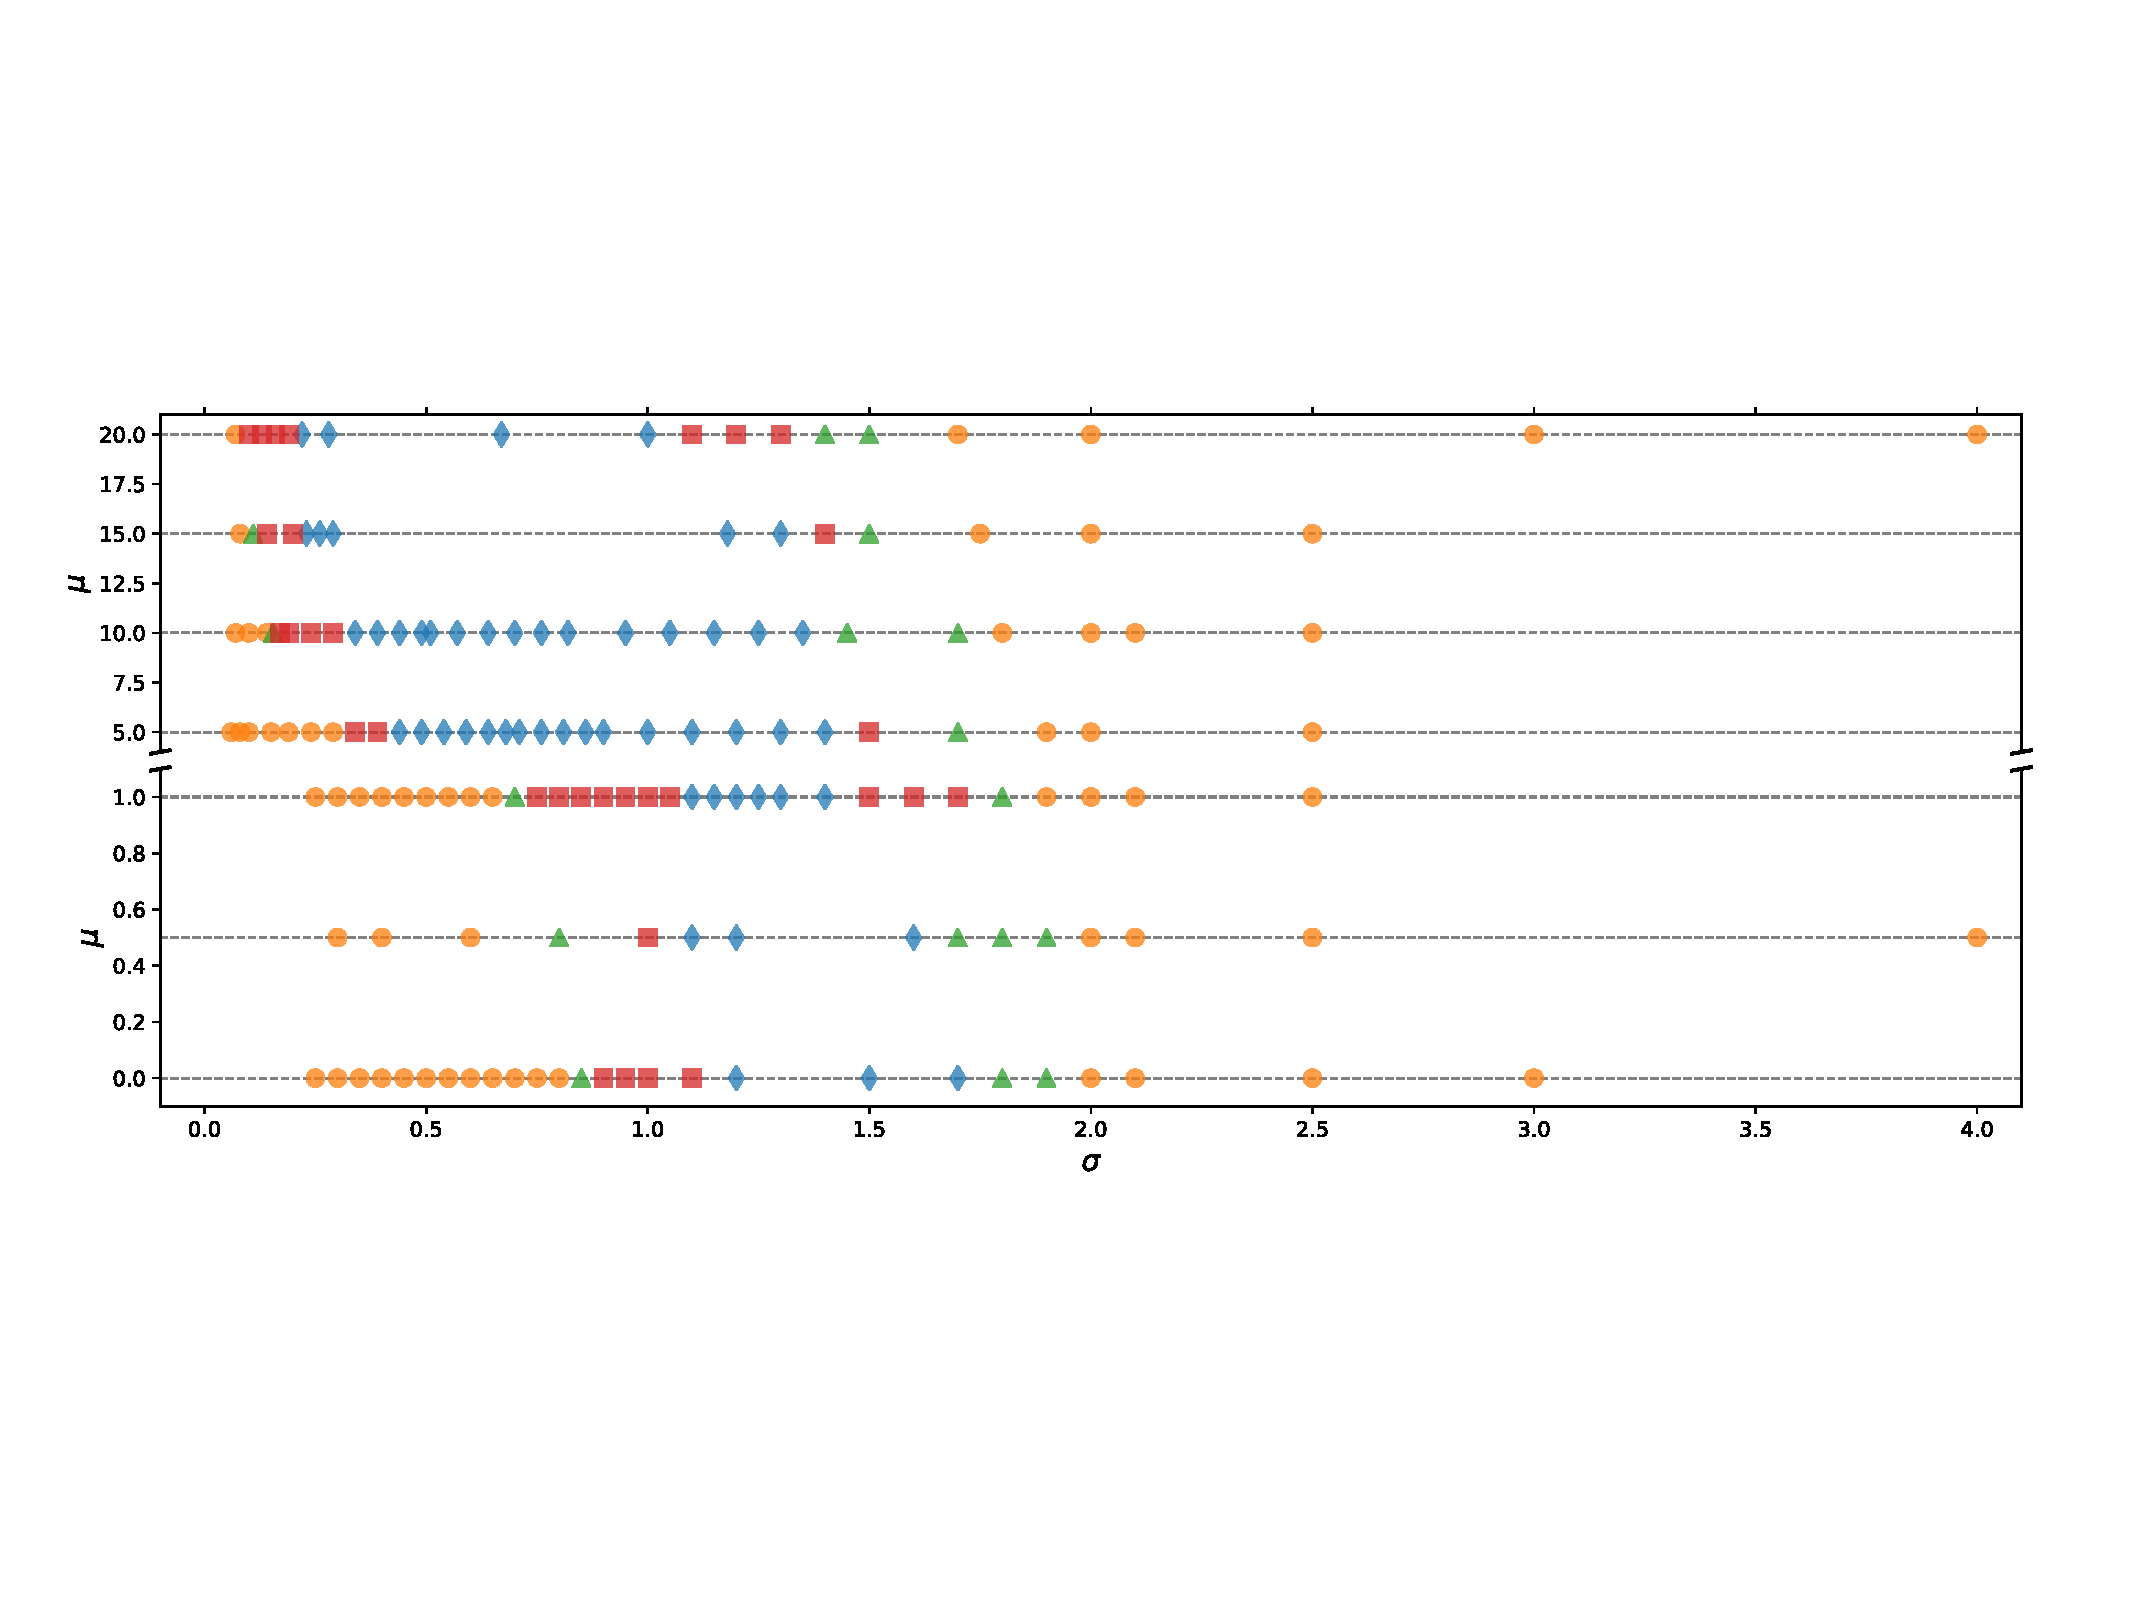
\includegraphics[width=\textwidth]{phase_plot}
  }
  \only<2>{
  \begin{center}
  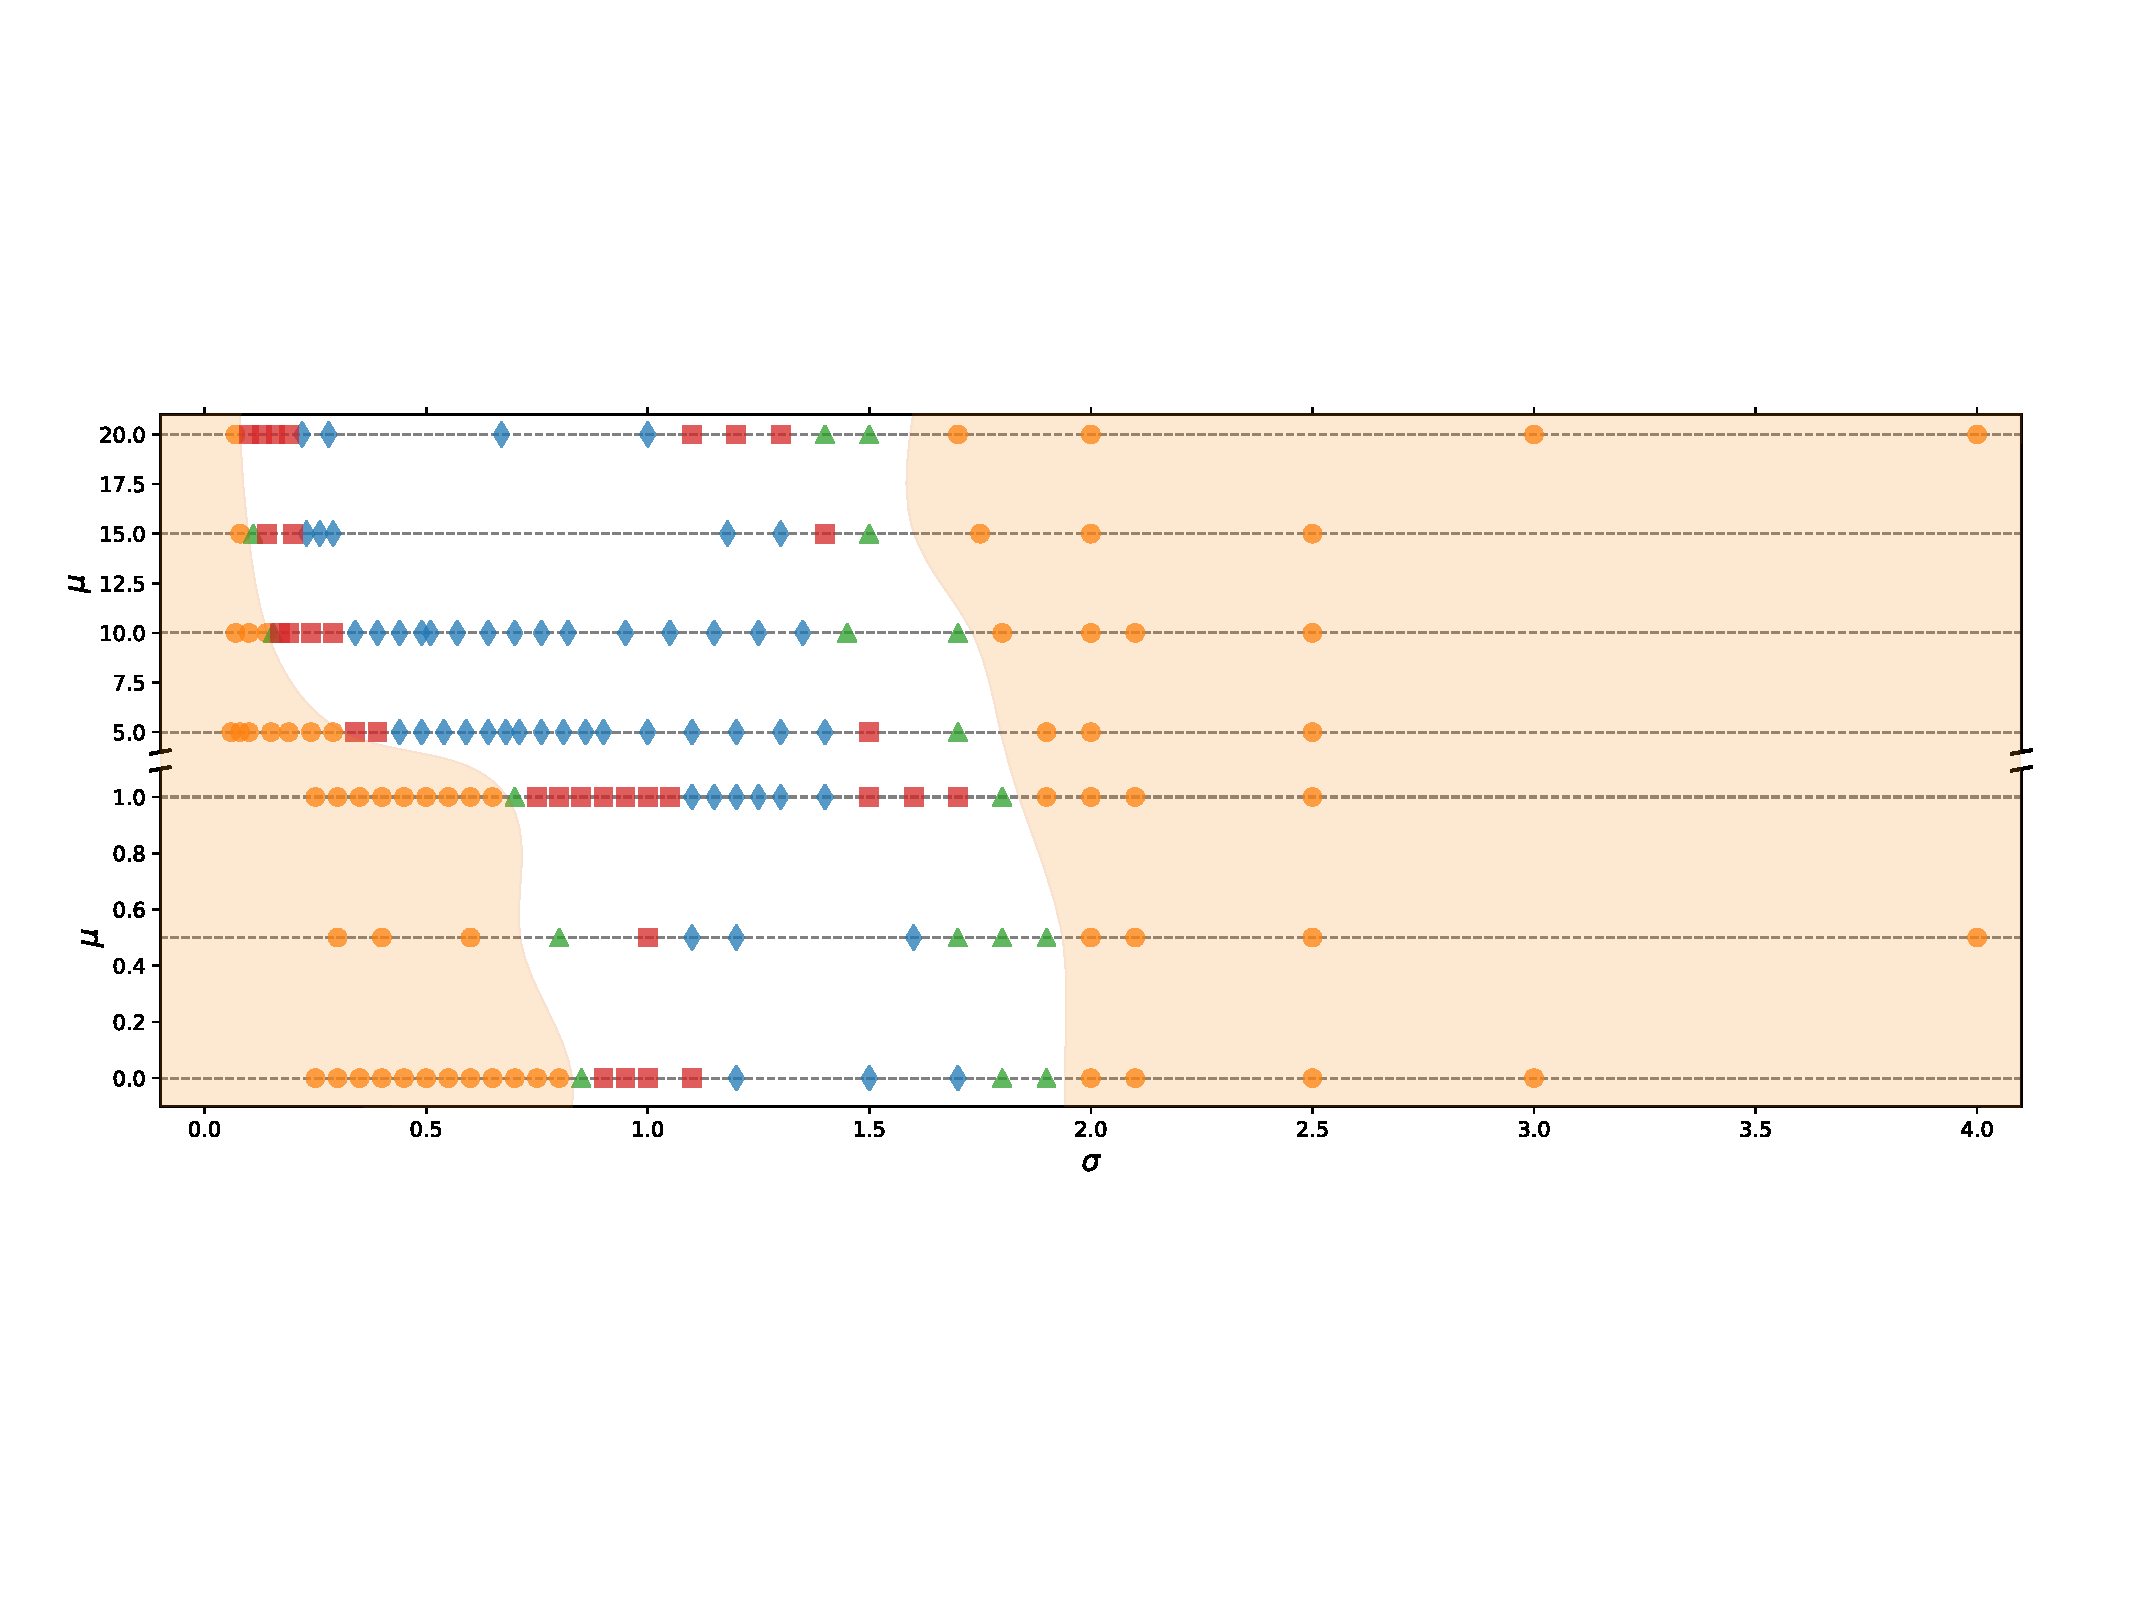
\includegraphics[width=\textwidth]{phase_sections1}
  \end{center}
  }
  \only<3>{
  \begin{center}
  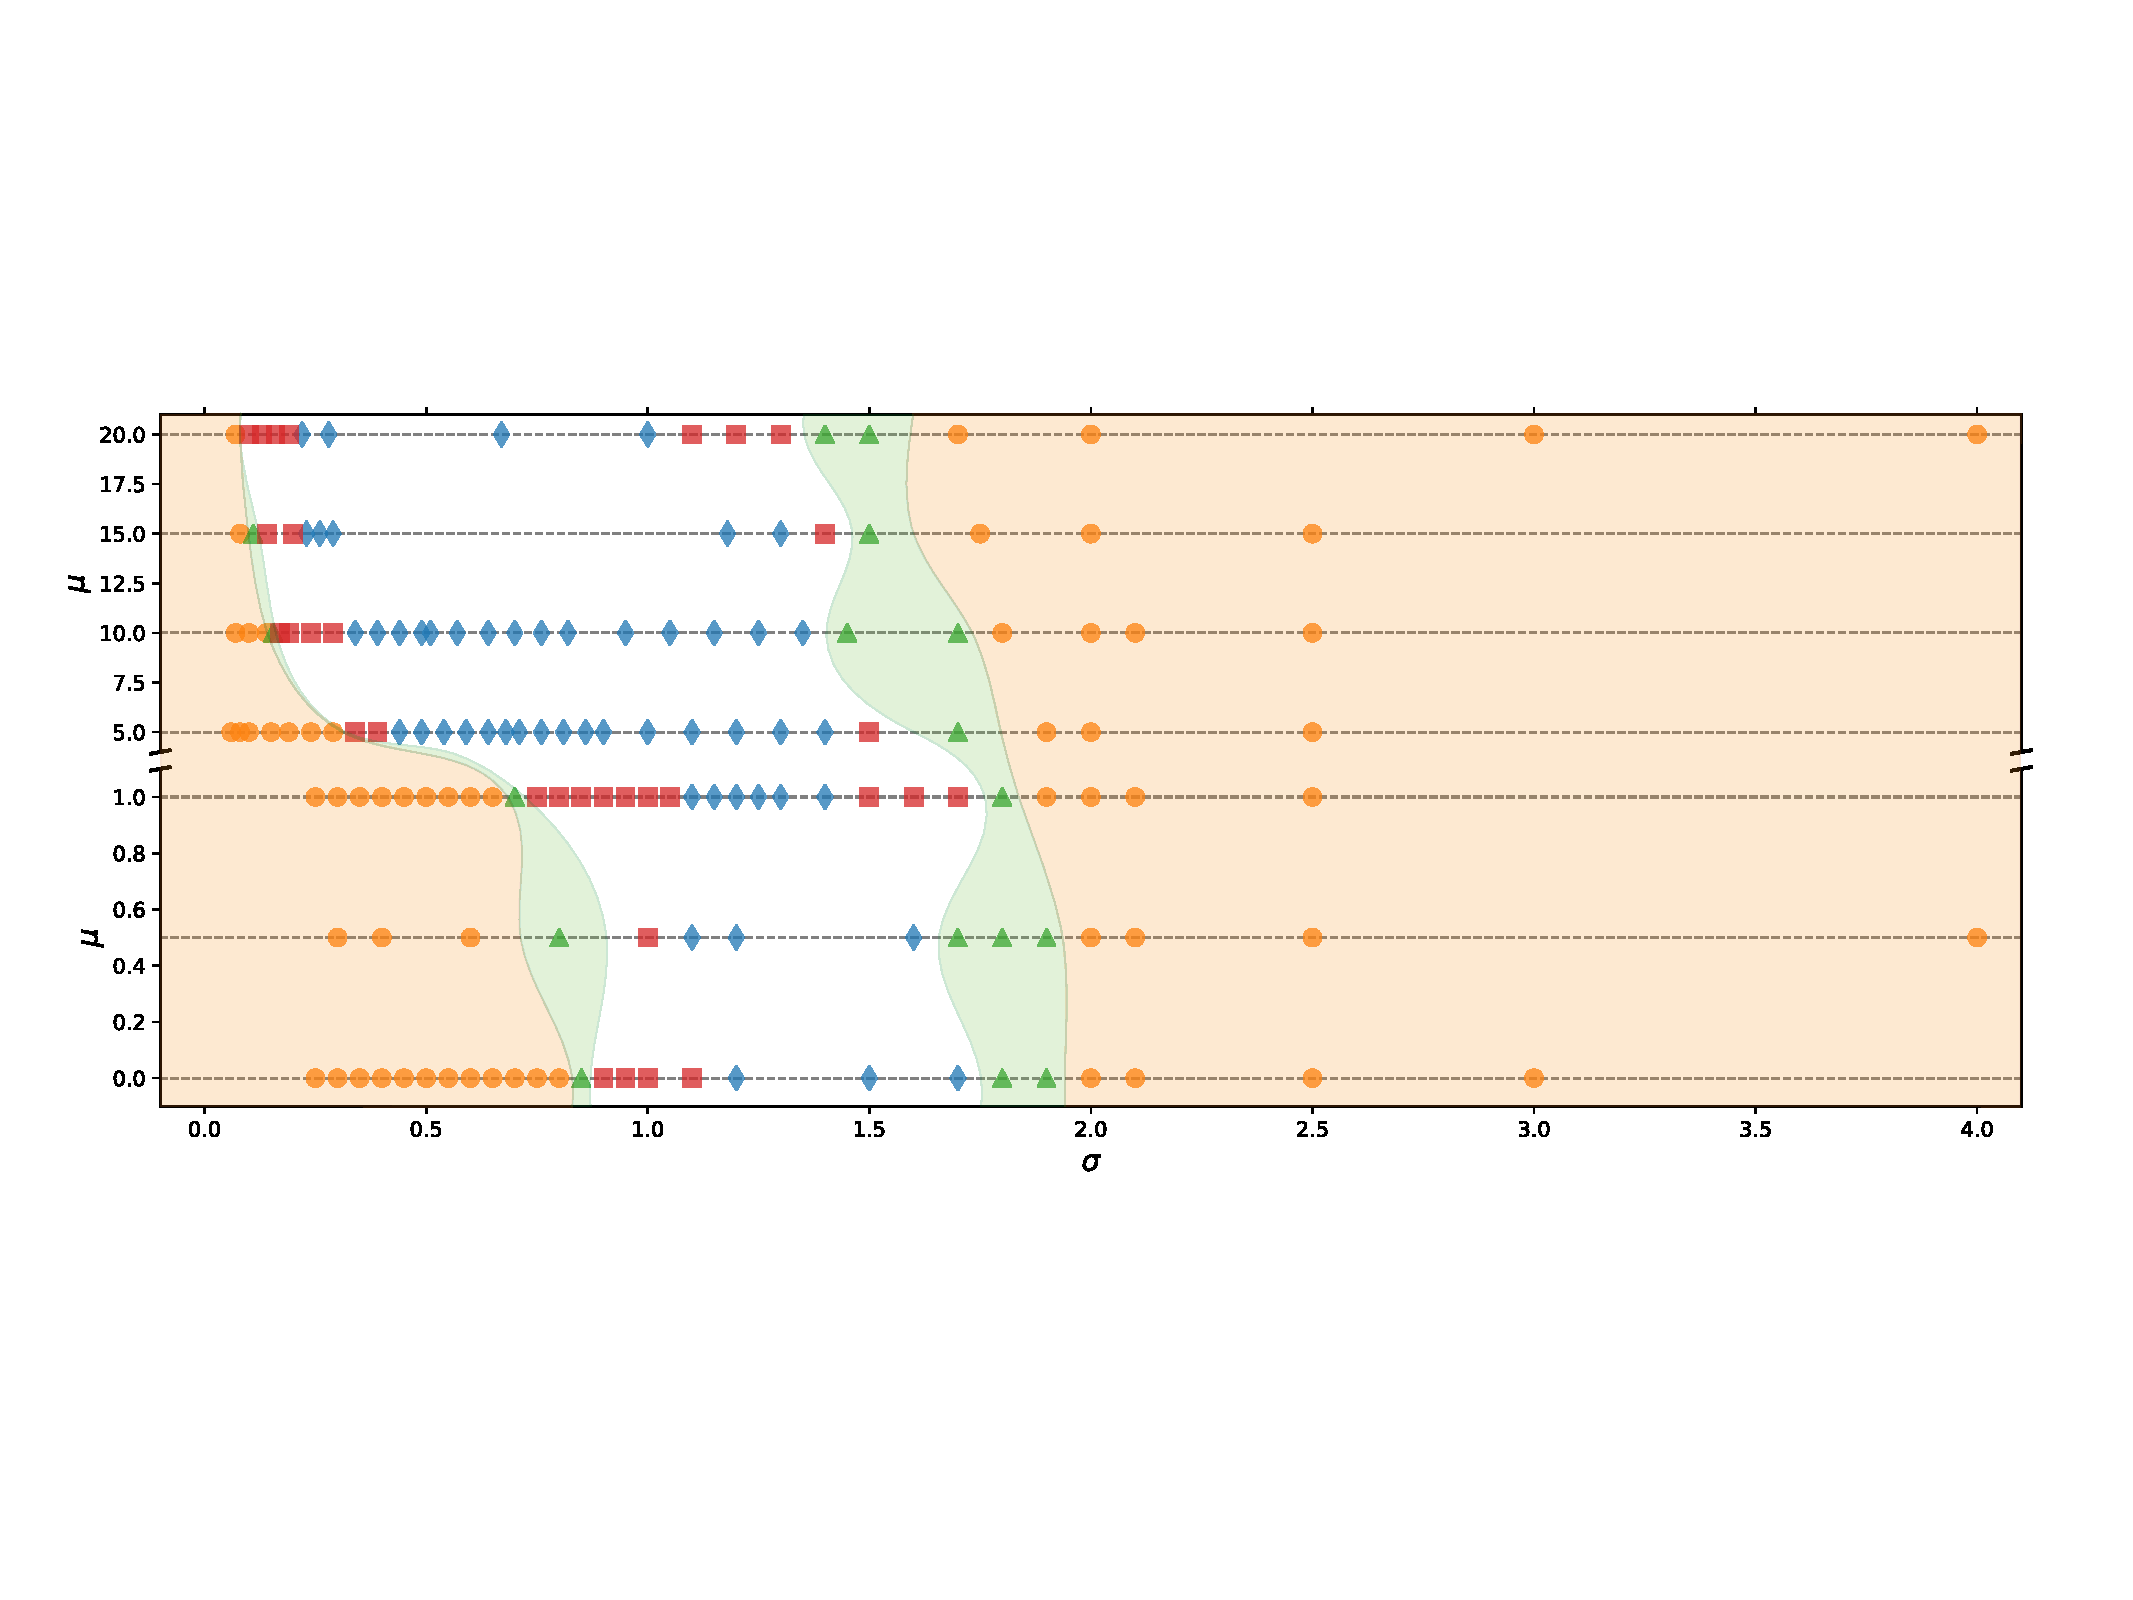
\includegraphics[width=\textwidth]{phase_sections2}
  \end{center}
  }
\only<4>{
  \begin{center}
  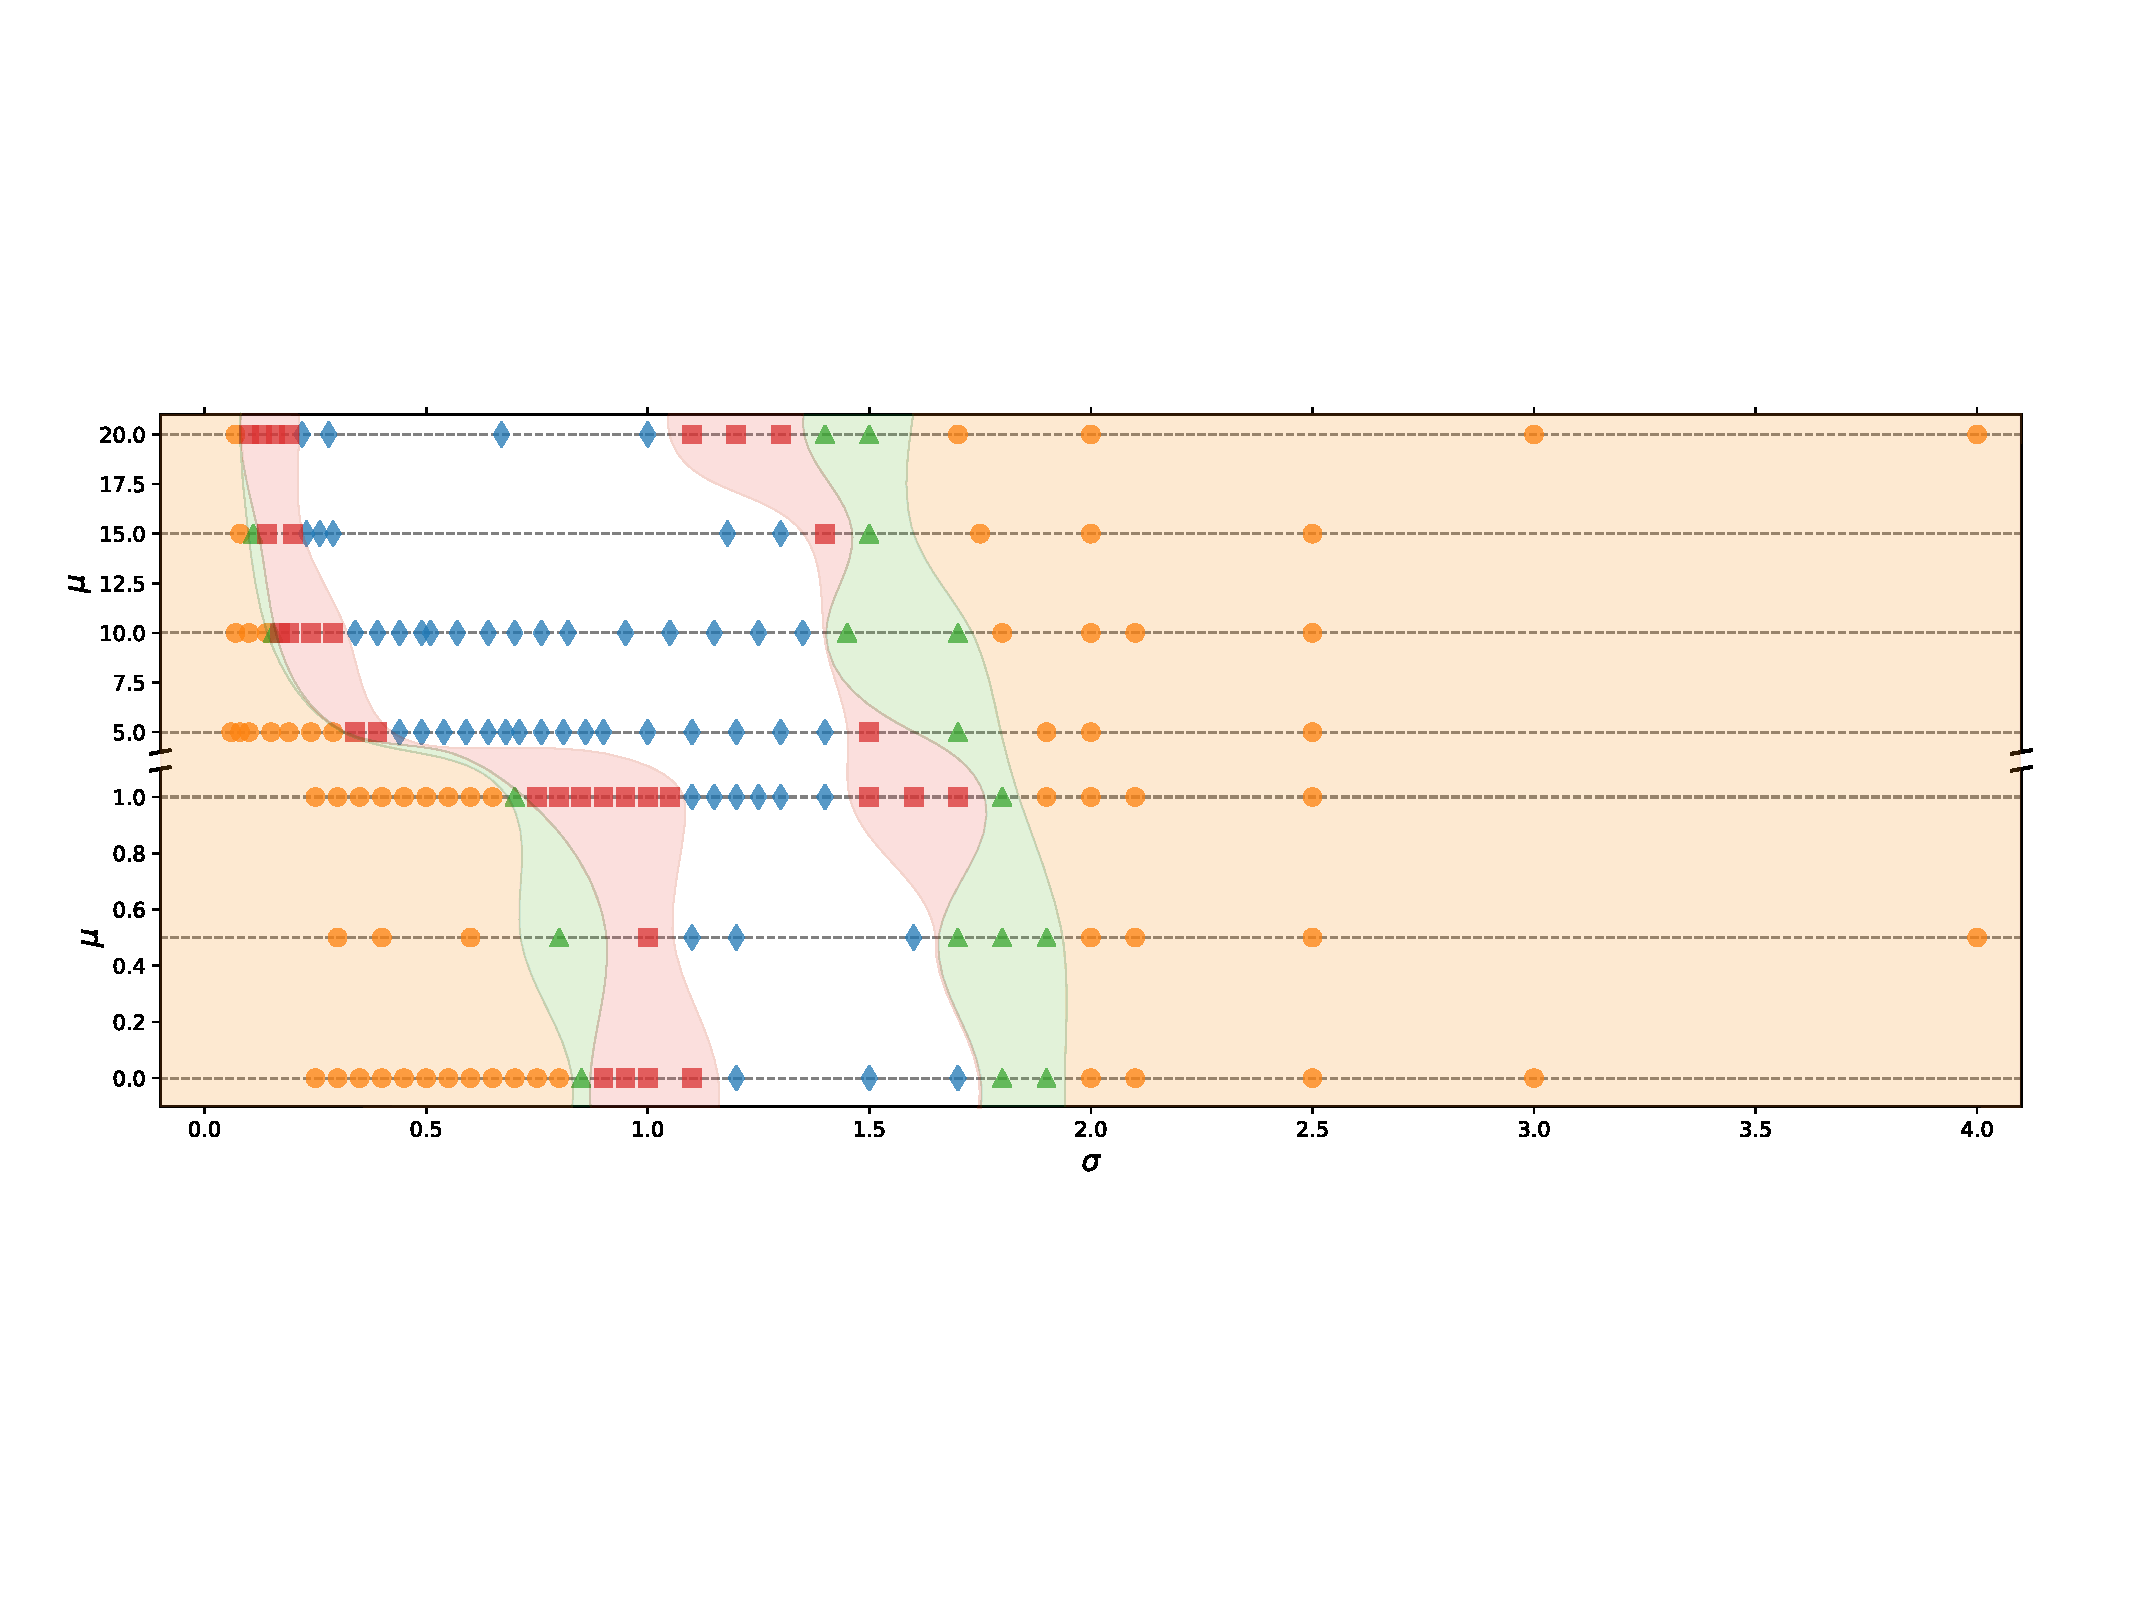
\includegraphics[width=\textwidth]{phase_sections3}
  \end{center}
  }
\only<5>{
  \begin{center}
  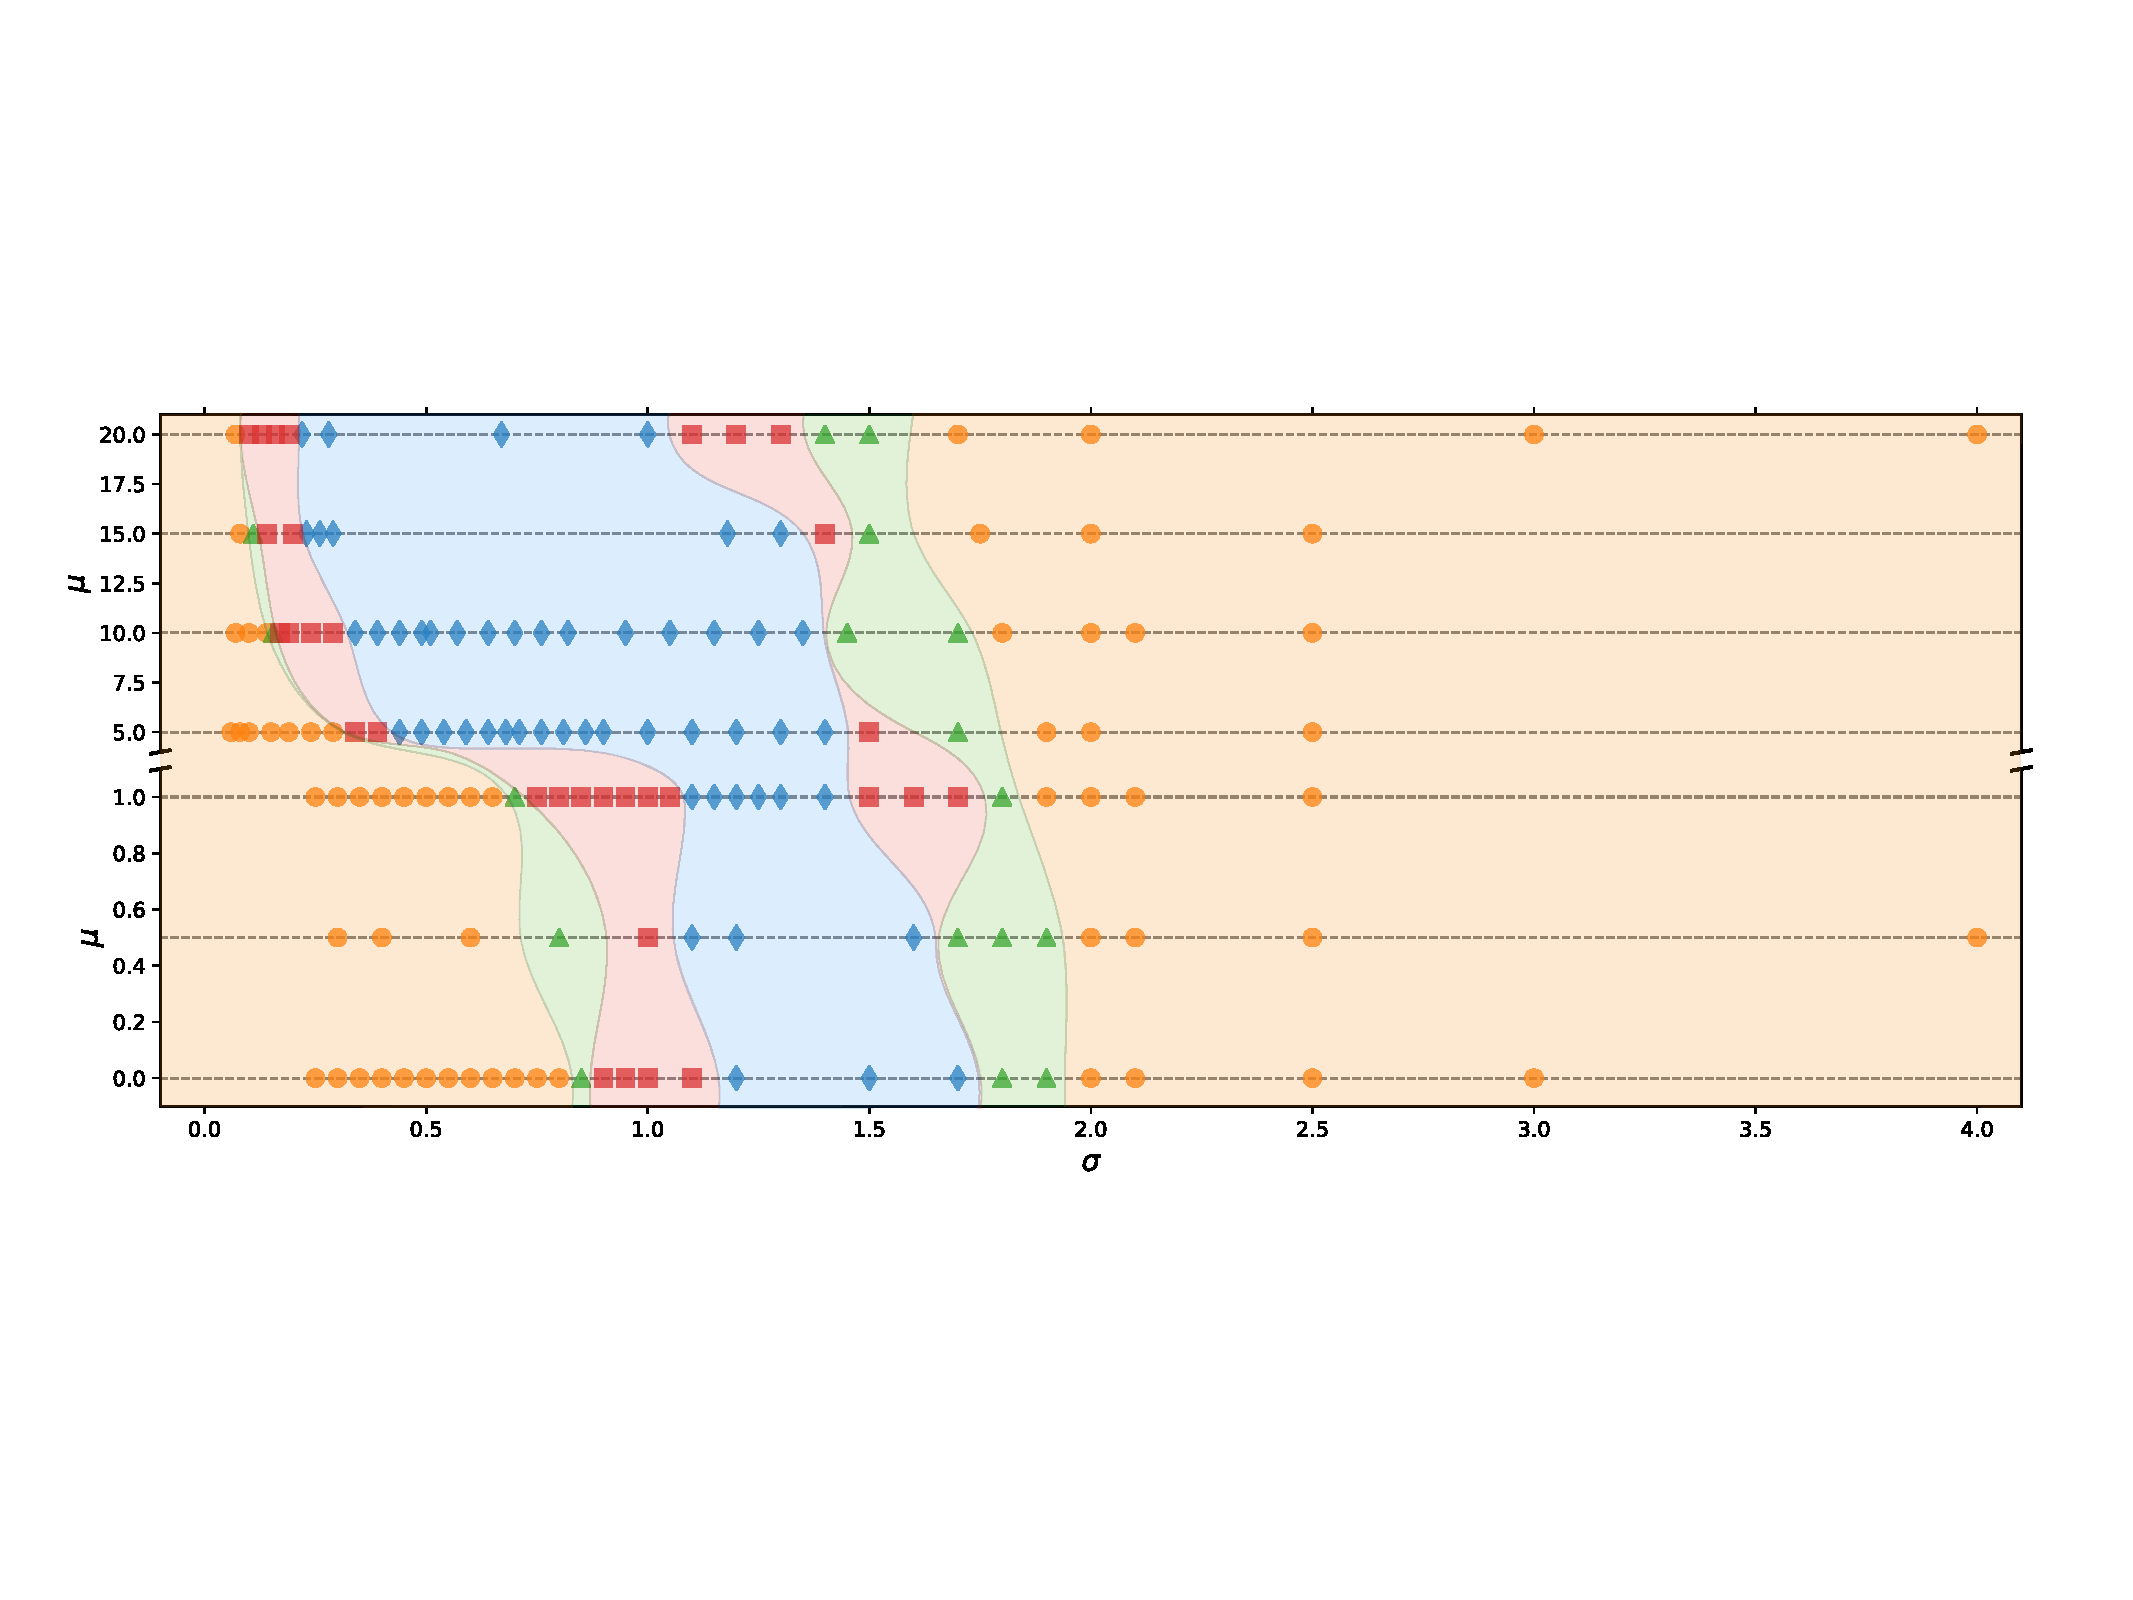
\includegraphics[width=\textwidth]{phase_sections4}
  \end{center}
  }
  \end{figure}
}

%%%%%%%%%%%%%%%%%%%%%%%%%%%%%%%%%%%%%%%%%%%%%%

\subsection{Phases}
\frame
{
  \frametitle{Unstable Profiles}
    \bi
    \its Fit $t_H \approx a \epsilon^{-p} + b$ $\to$ unstable when $p \approx 2$
    \its<2->{$\sigma < 1$: $a \sim \sigma^{-2}$, mass independent}
    \ei
    \begin{columns}
    \column{0.5\textwidth}  
      \begin{figure}
      \centering
      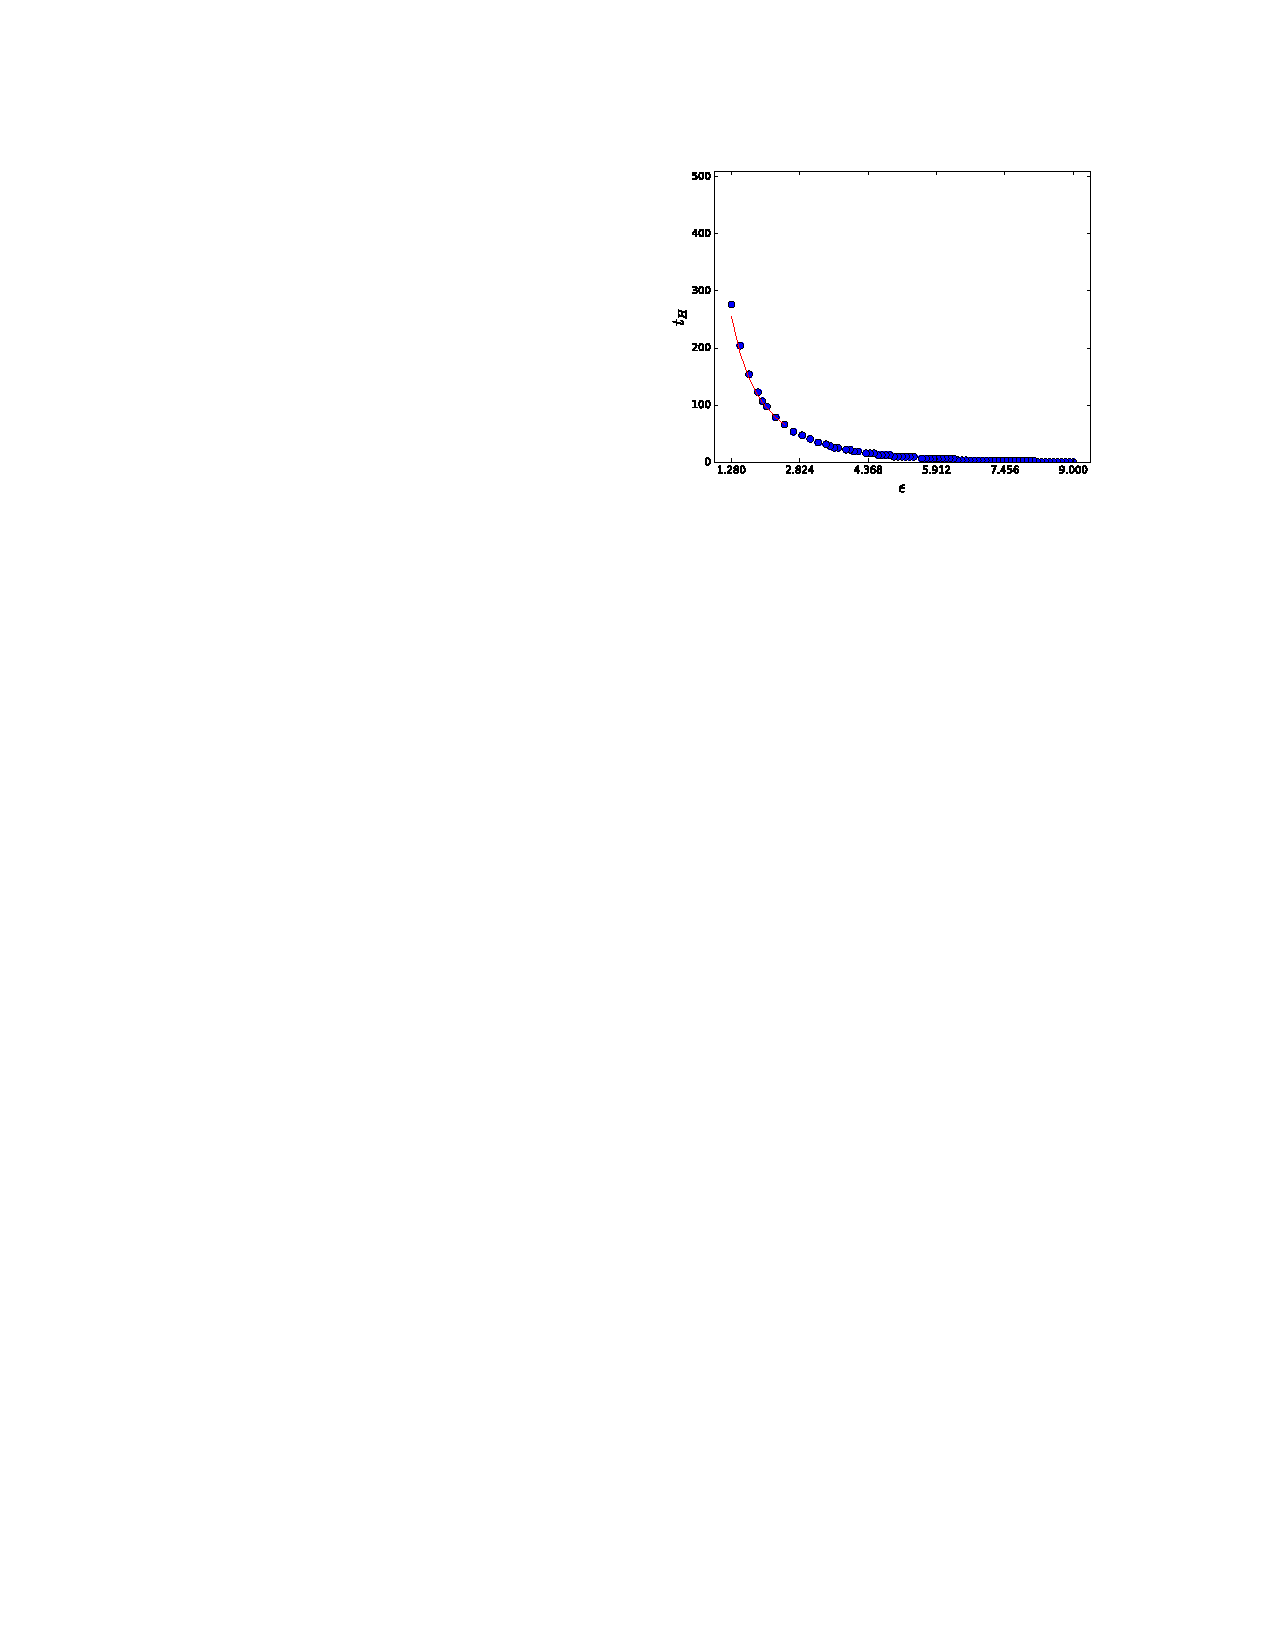
\includegraphics[scale=0.75]{m0w025} \\ $\mu = 5$, $\sigma=0.25$
      \end{figure}
    \column{0.5\textwidth}
      \begin{figure}
      \centering
      \hspace{-0.2in}
      \vspace{0.2in}
      \uncover<2->{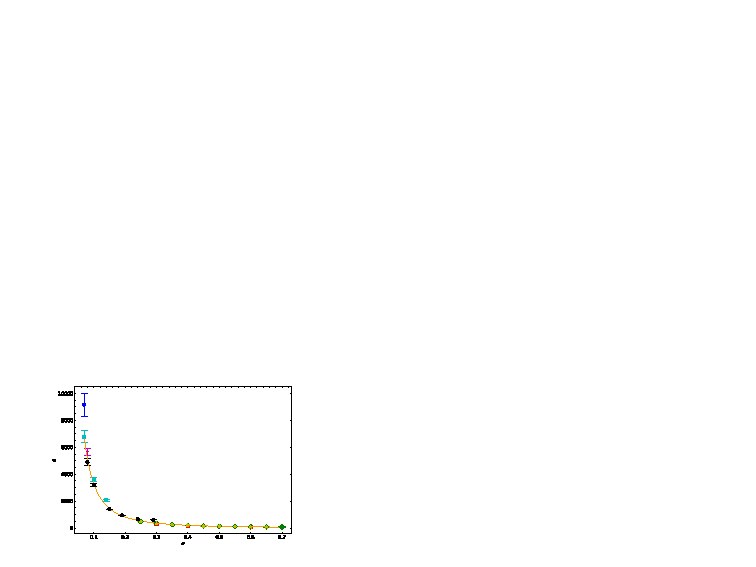
\includegraphics[scale=1.5]{coefficientscaling}}
      \end{figure}
    \end{columns}
}

\frame
{
  \frametitle{Metastable Profiles}
  \bi
  \its Scaling of $p > 2$
  \ei
  \begin{columns}
  \column{0.5\textwidth}
    \begin{figure}
    \centering
    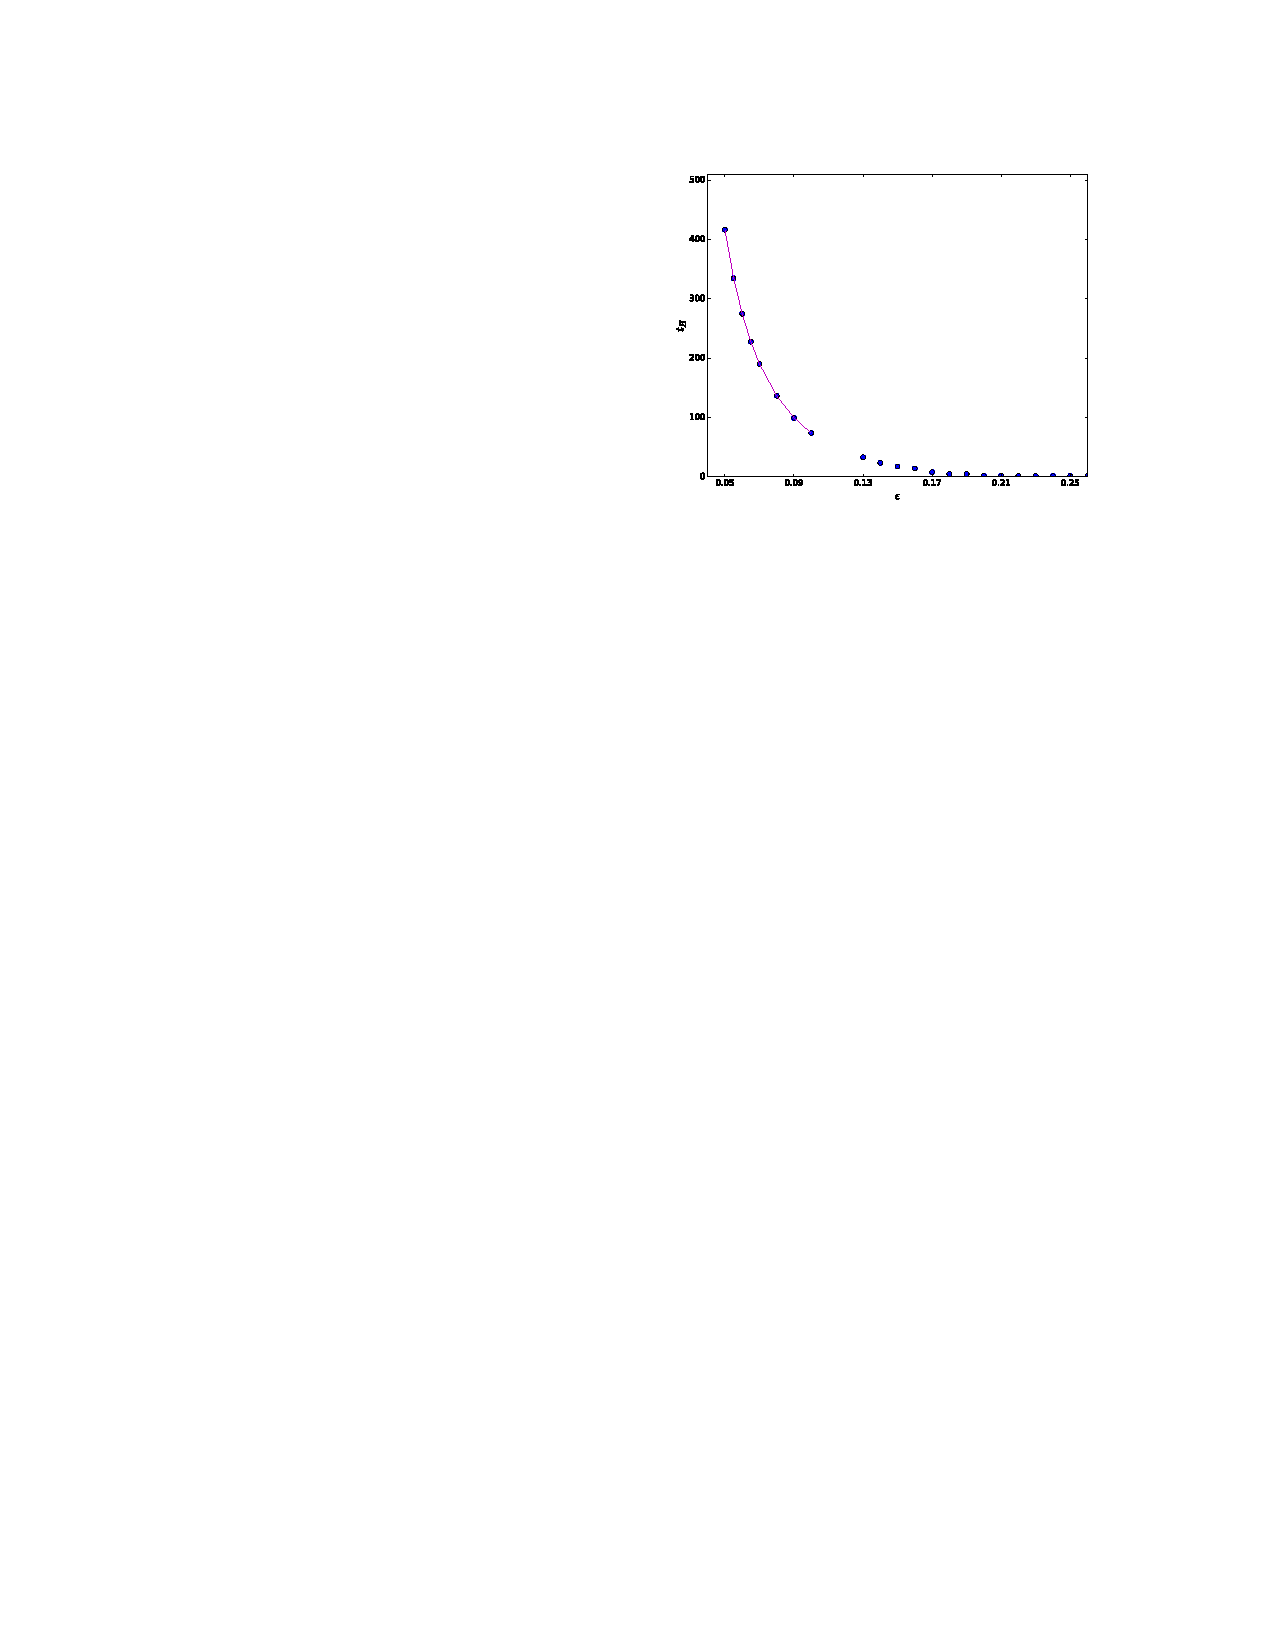
\includegraphics[scale=0.75]{m5w17} \\ $\mu = 5$, $\sigma = 1.7$
    \end{figure}
  \column{0.5\textwidth}
    \begin{figure}
    \centering
    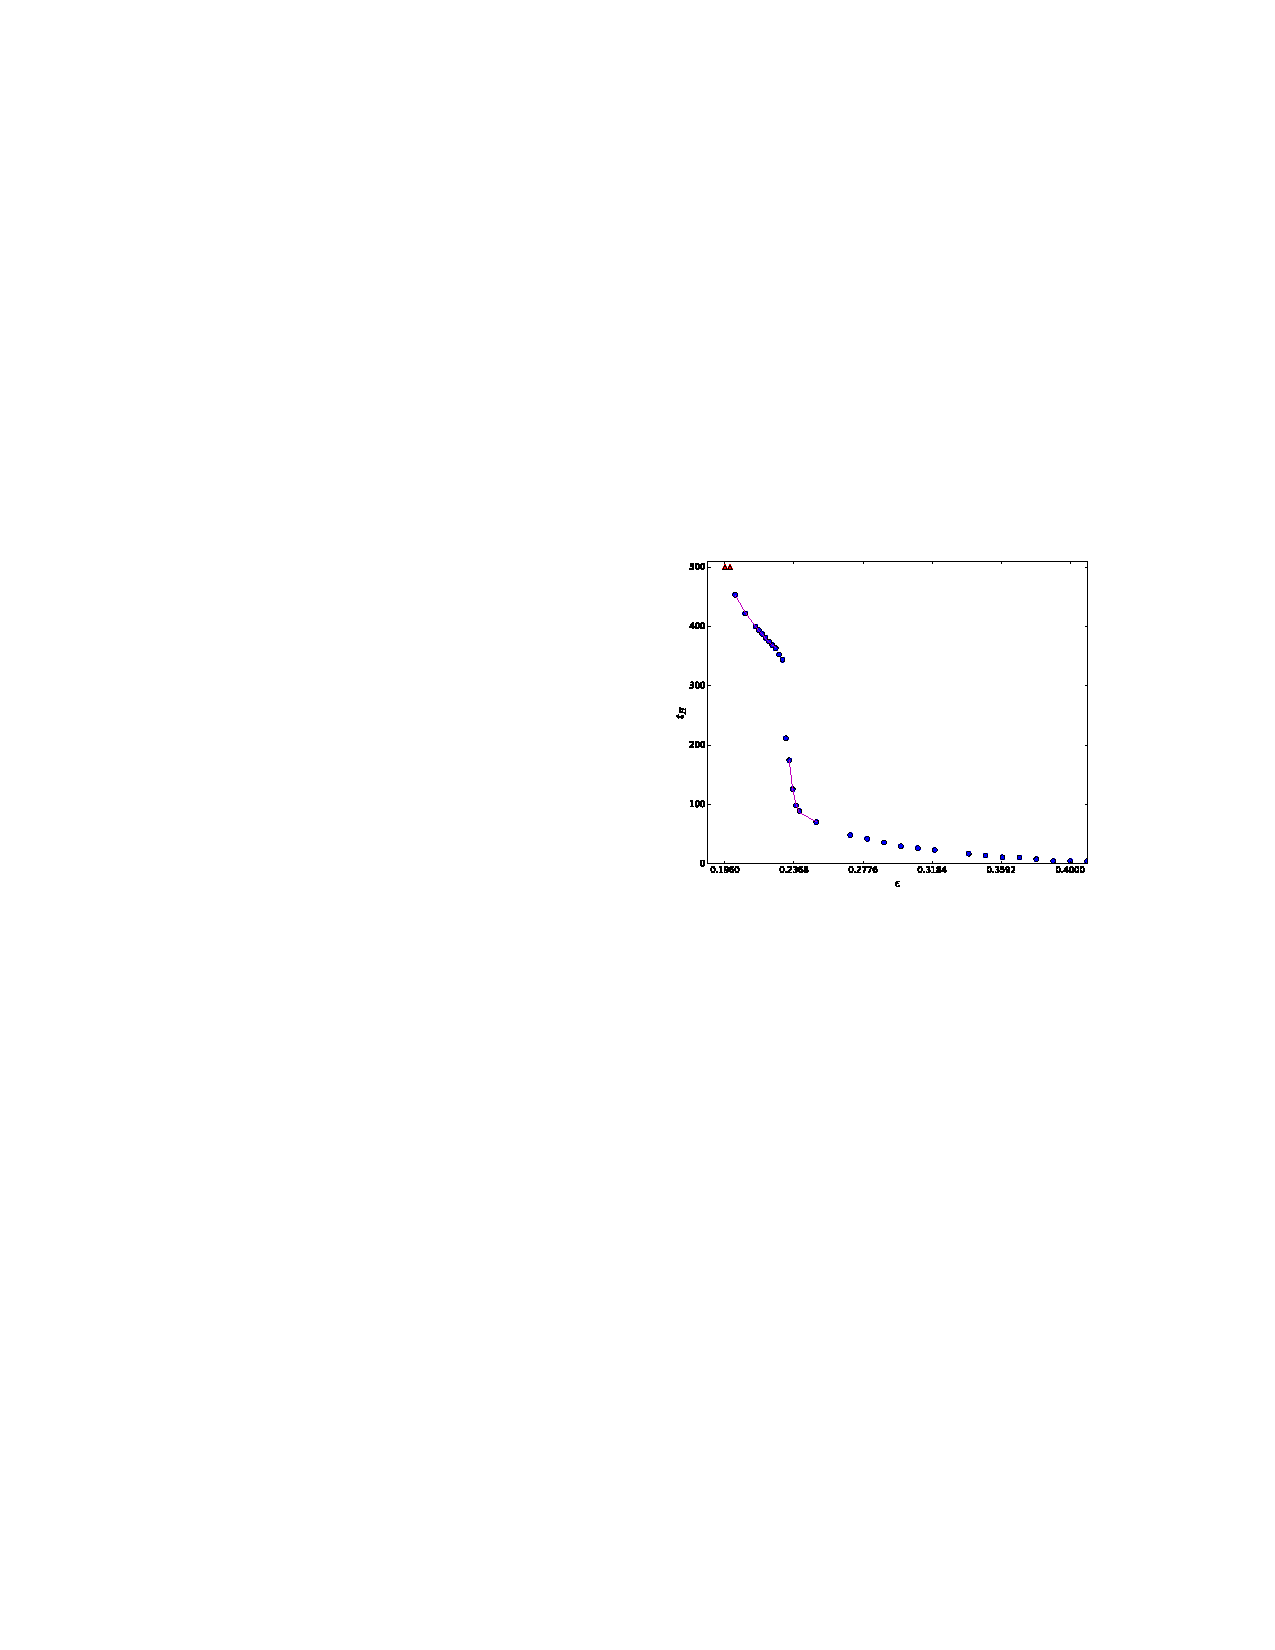
\includegraphics[scale=0.75]{m05w17} \\ $\mu = 0.5$, $\sigma = 1.7$
    \end{figure}
  \end{columns}
}

\frame
{
  \frametitle{Irregular Profiles}
  \only<1>{
  \bi
  \its No scaling
  \ei
  \begin{columns}
  \column{0.45\textwidth}
  	\begin{figure}
  	\centering
  	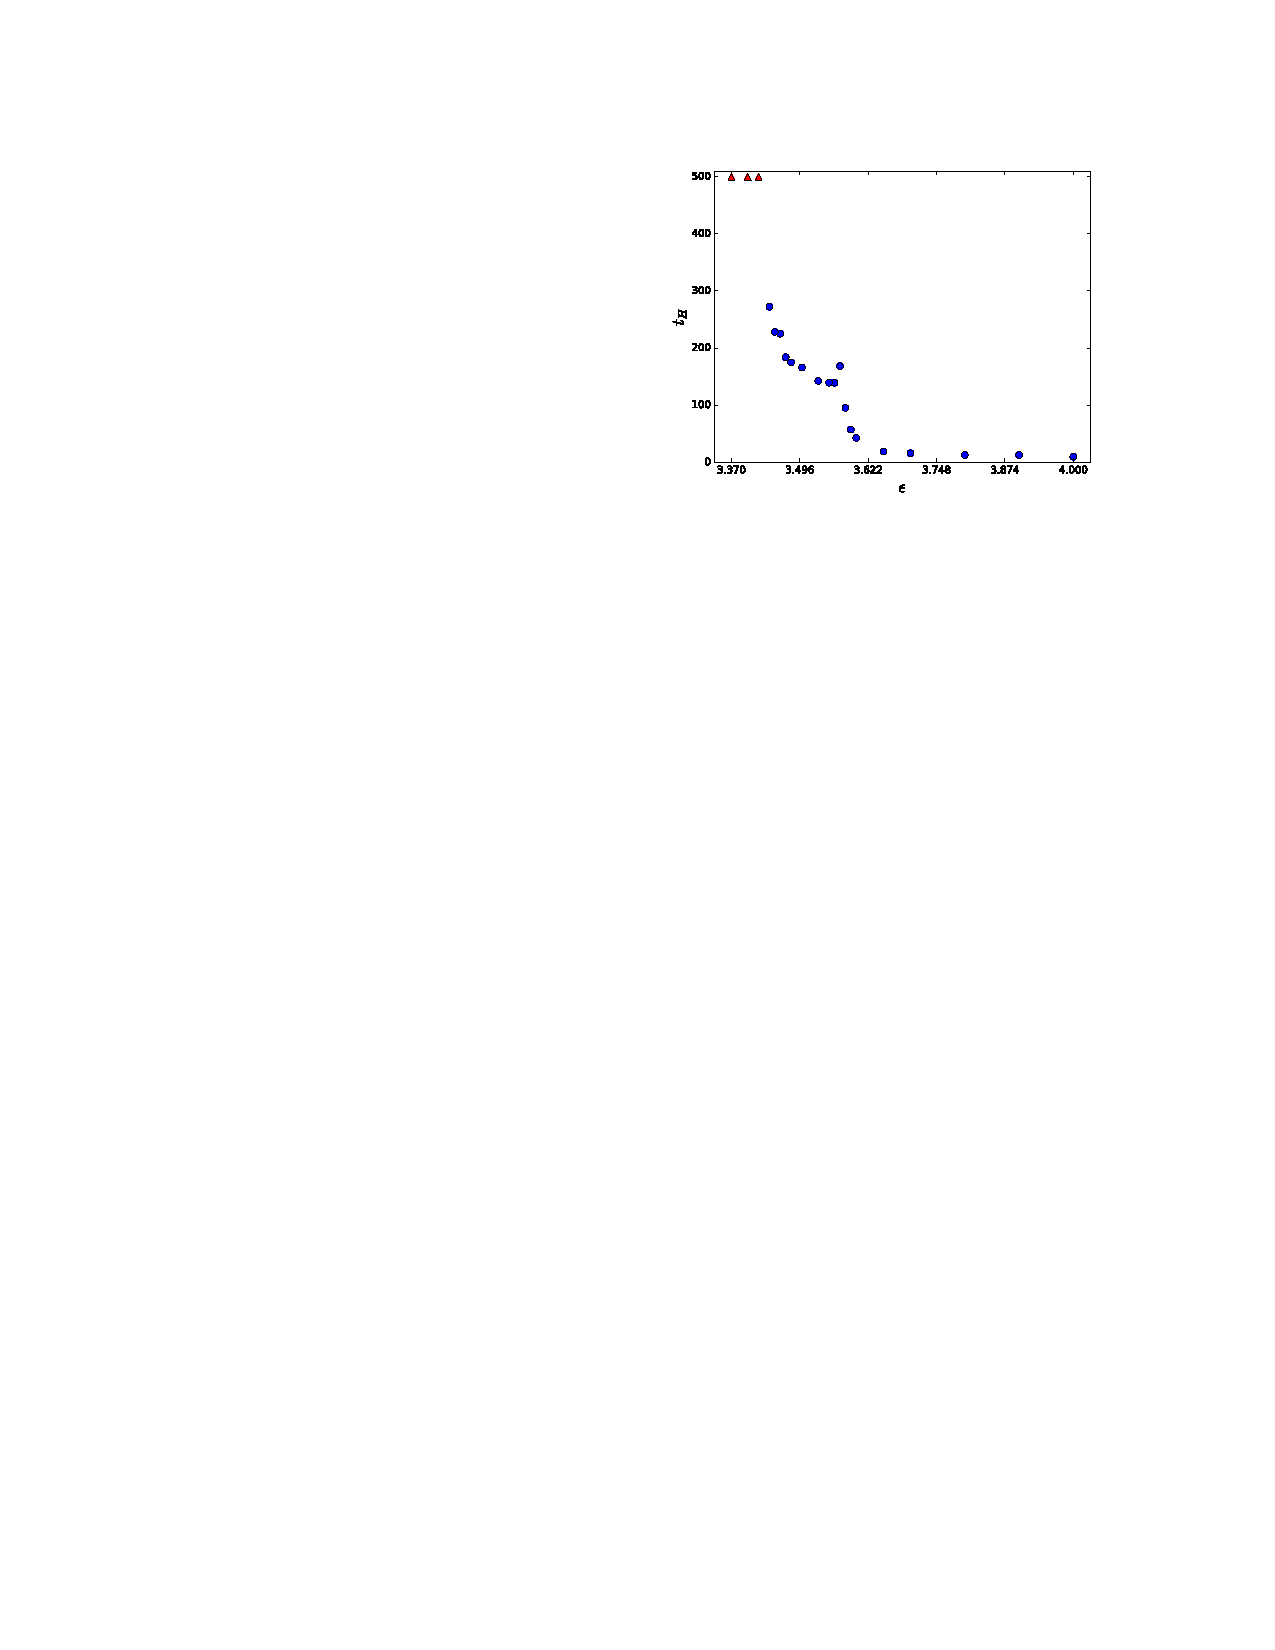
\includegraphics[width=\textwidth]{m5w034} \\ $\mu = 5$, $\sigma = 0.34$
  	\end{figure}
  \column{0.45\textwidth}
  	\begin{figure}
	\centering
	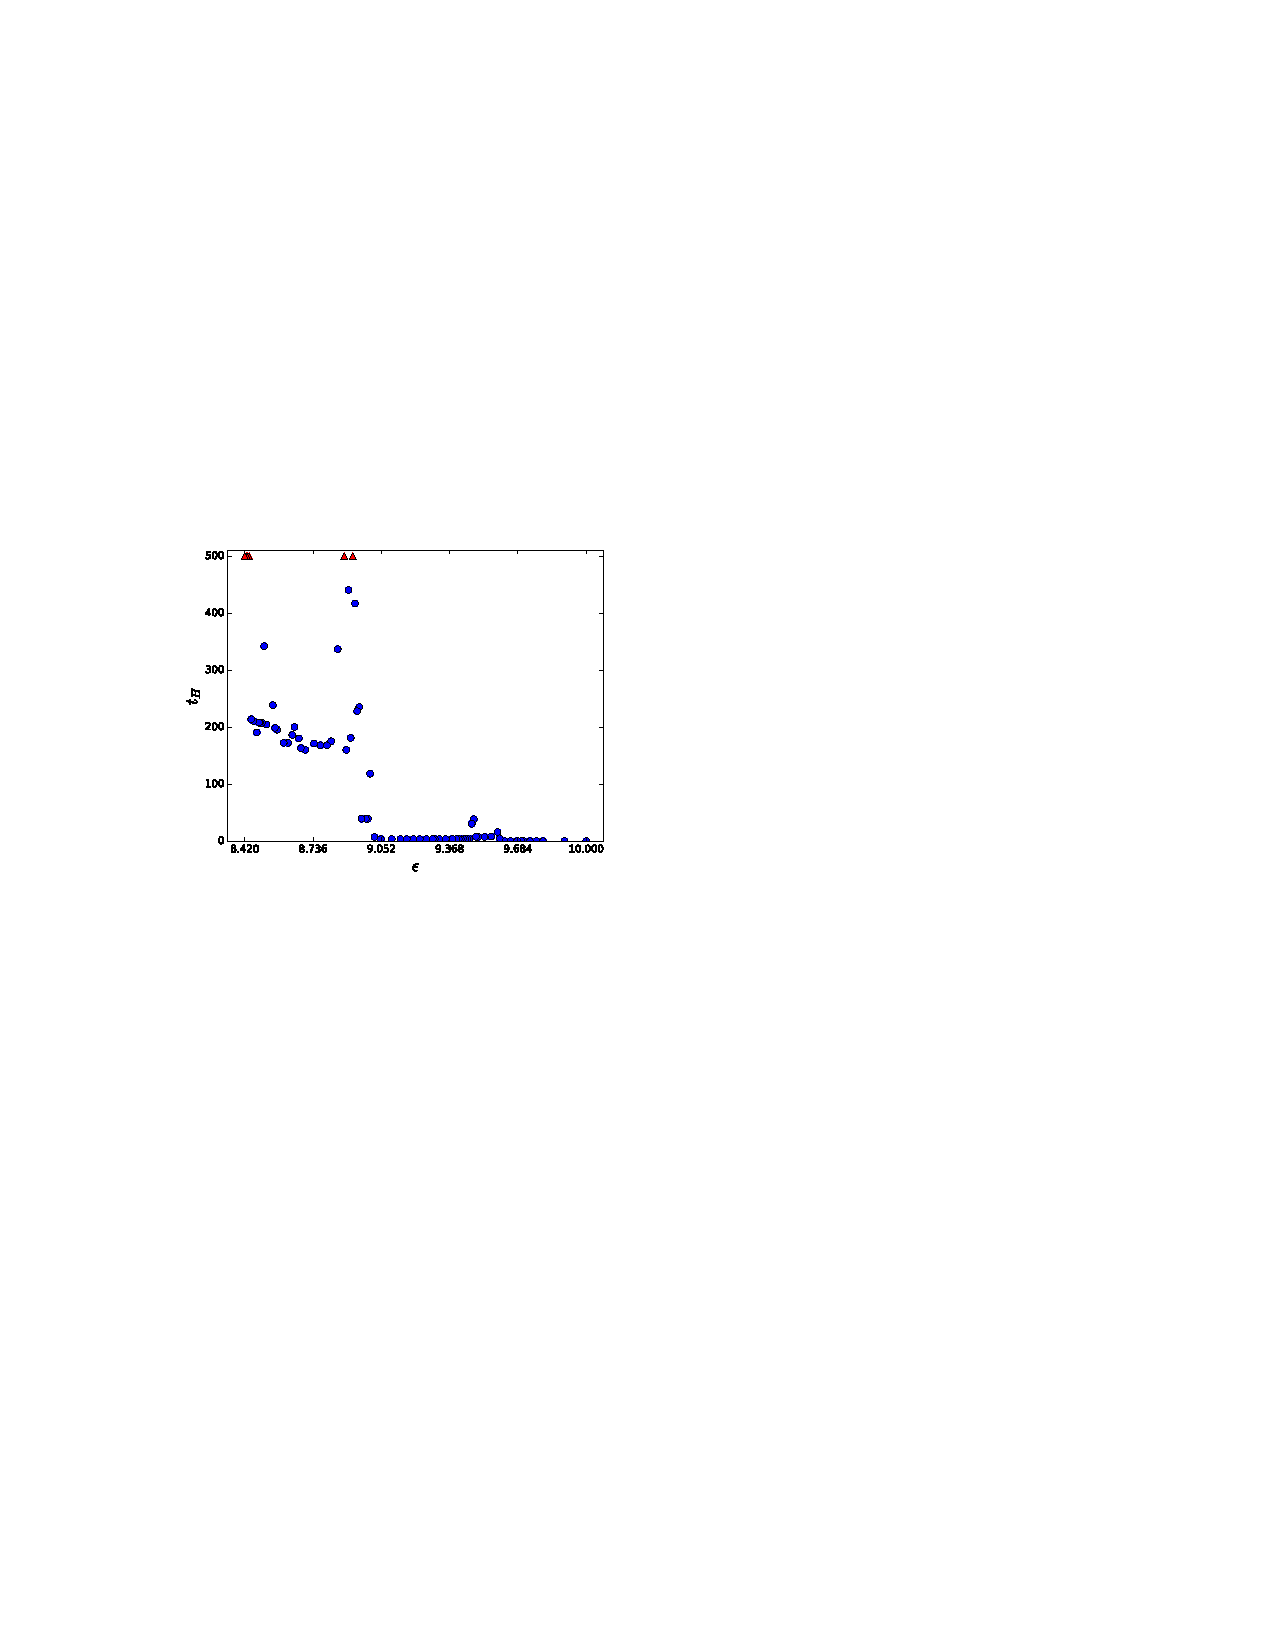
\includegraphics[width=\textwidth]{m20w016} \\ $\mu = 20$, $\sigma = 0.16$
  	\end{figure}
  \end{columns}
  }
  \only<2>{
  \bi
  \its Evidence of chaotic behaviour $\to$ possible \alert{self-interaction}
  \its Previous chaotic evolution only seen in thin-shell interactions\footnotemark\ in AdS, scalar collapse in Gauss-Bonnet gravity\footnotemark
  \ei
  \begin{figure}
  	\centering
	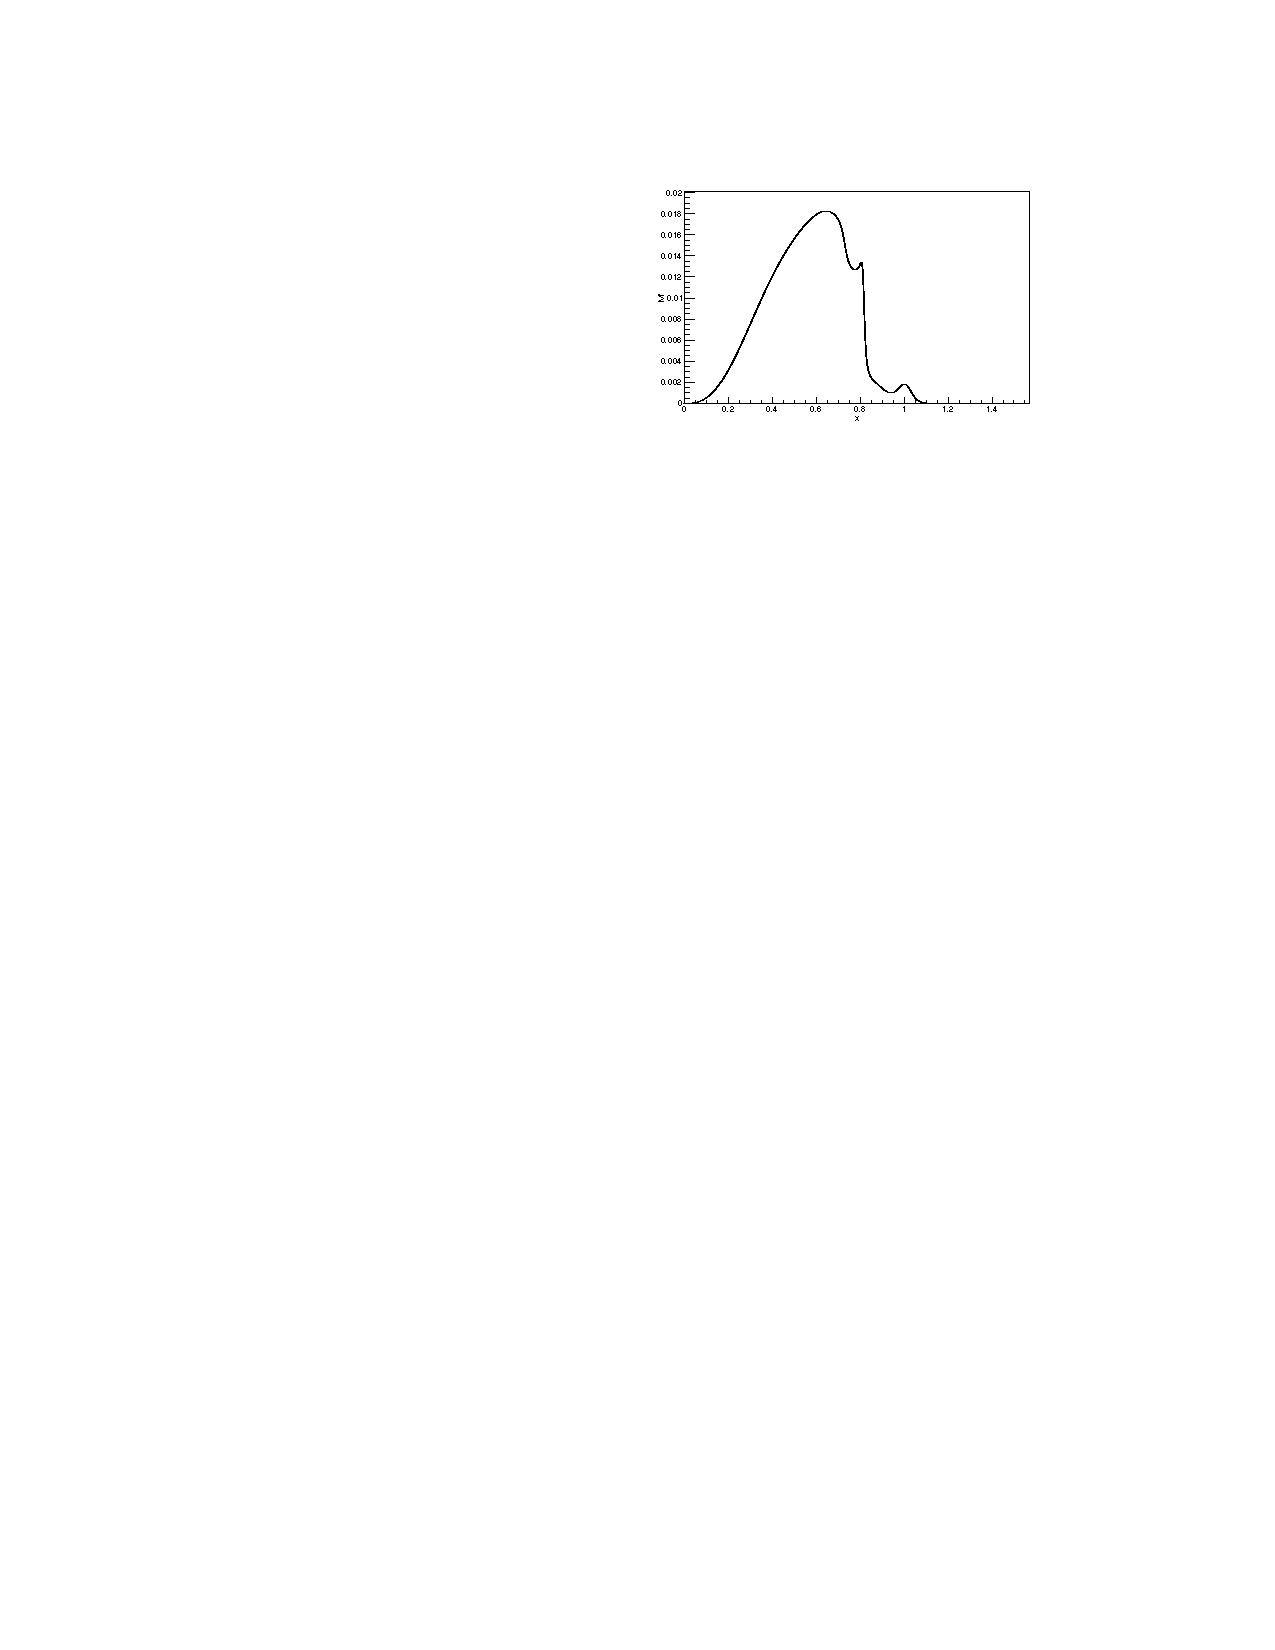
\includegraphics[scale=1.0]{chaotic} \\ $\mu = 5$, $\sigma=0.34$, $\epsilon = 3.52$, $t = 137$
  \end{figure}
  
  \footnotetext[5]{{\scr Brito {\it et al.} [1602.03535]}}
  \footnotetext[6]{{\scr Deppe, Kolly, {\it et al.} [1608.05402]}}
  }
}

\frame
{
  \frametitle{Energy Cascades}
  \bi
  \its Stable solutions: \alert{direct} and \alert{inverse} energy cascades
  \ei
  \begin{columns}
  \column{0.5\textwidth}
      \begin{figure}
      \centering
      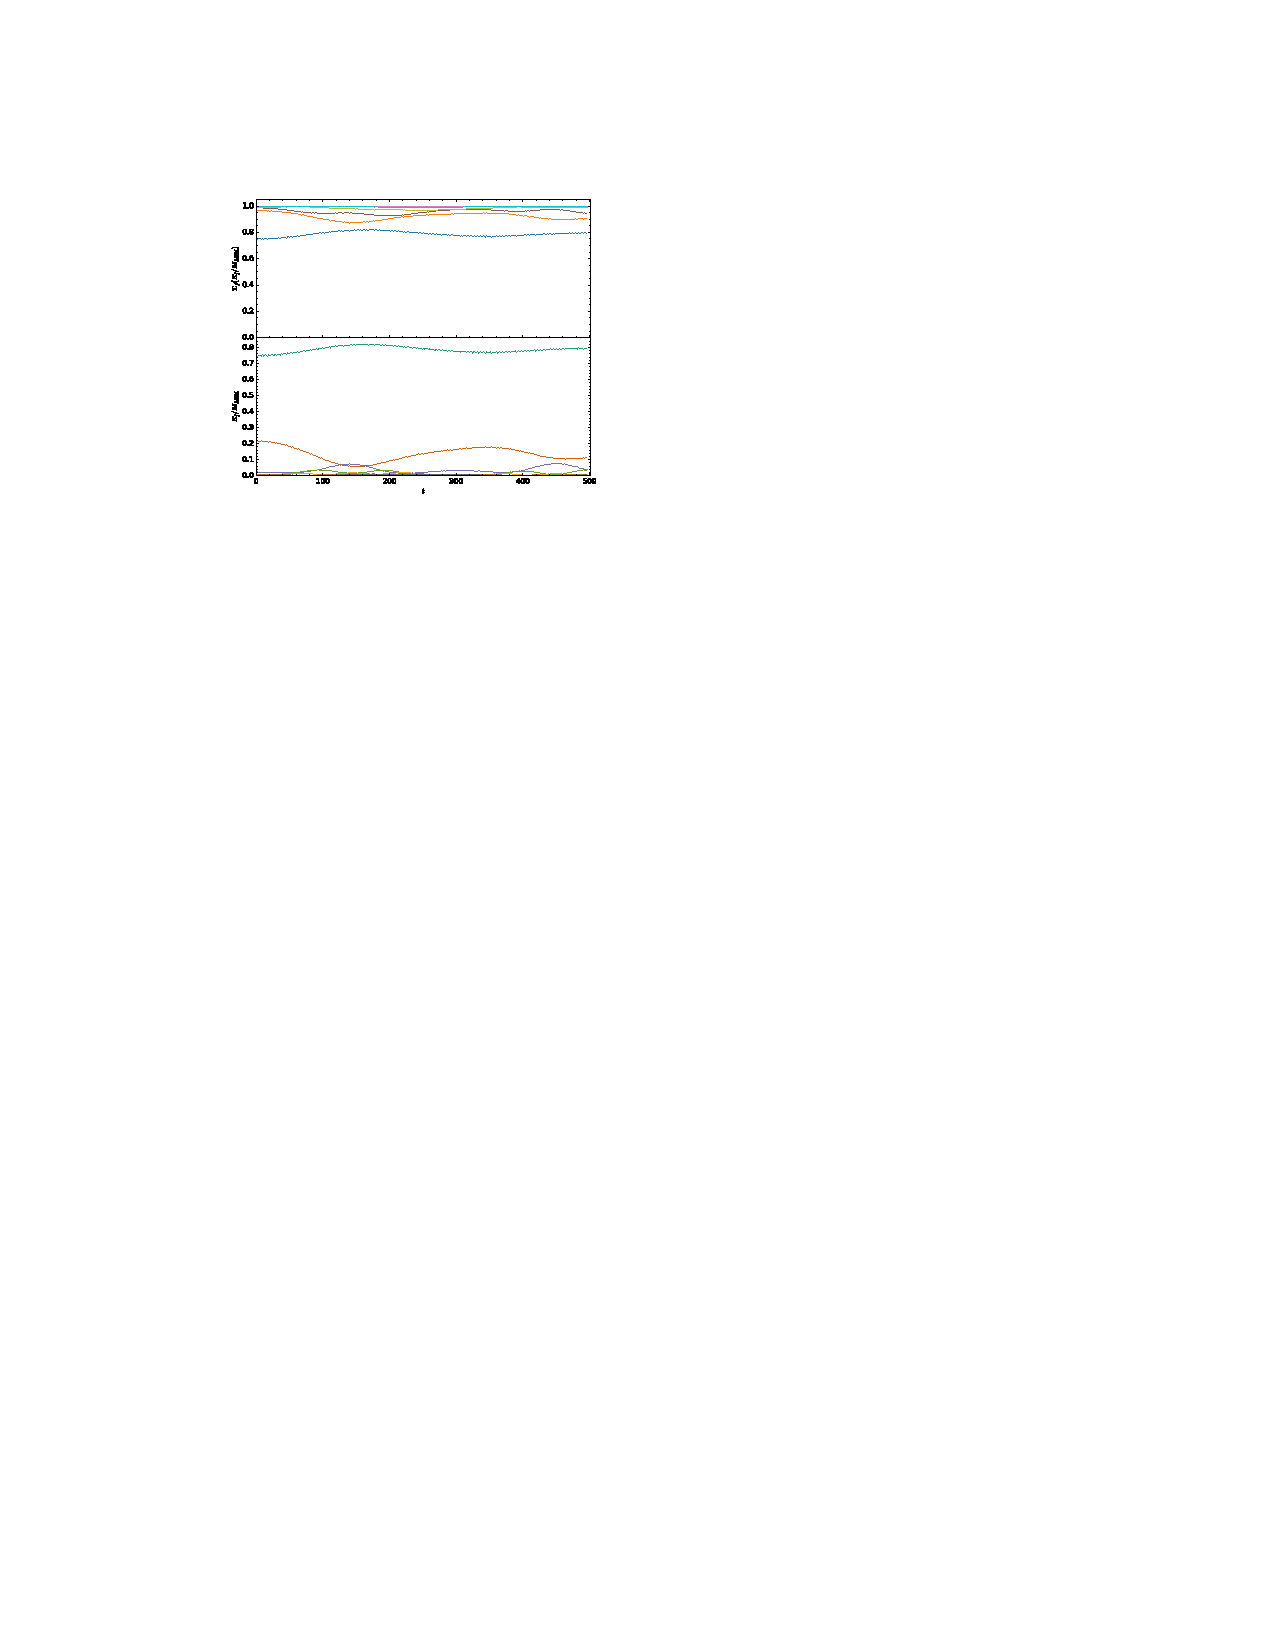
\includegraphics[width=\textwidth]{Em0w18} \\ $\mu = 0$, $\sigma = 1.8$, $\epsilon=0.13$ \\ Stable
      \end{figure}
  \column{0.5\textwidth}
      \begin{figure}
      \centering
      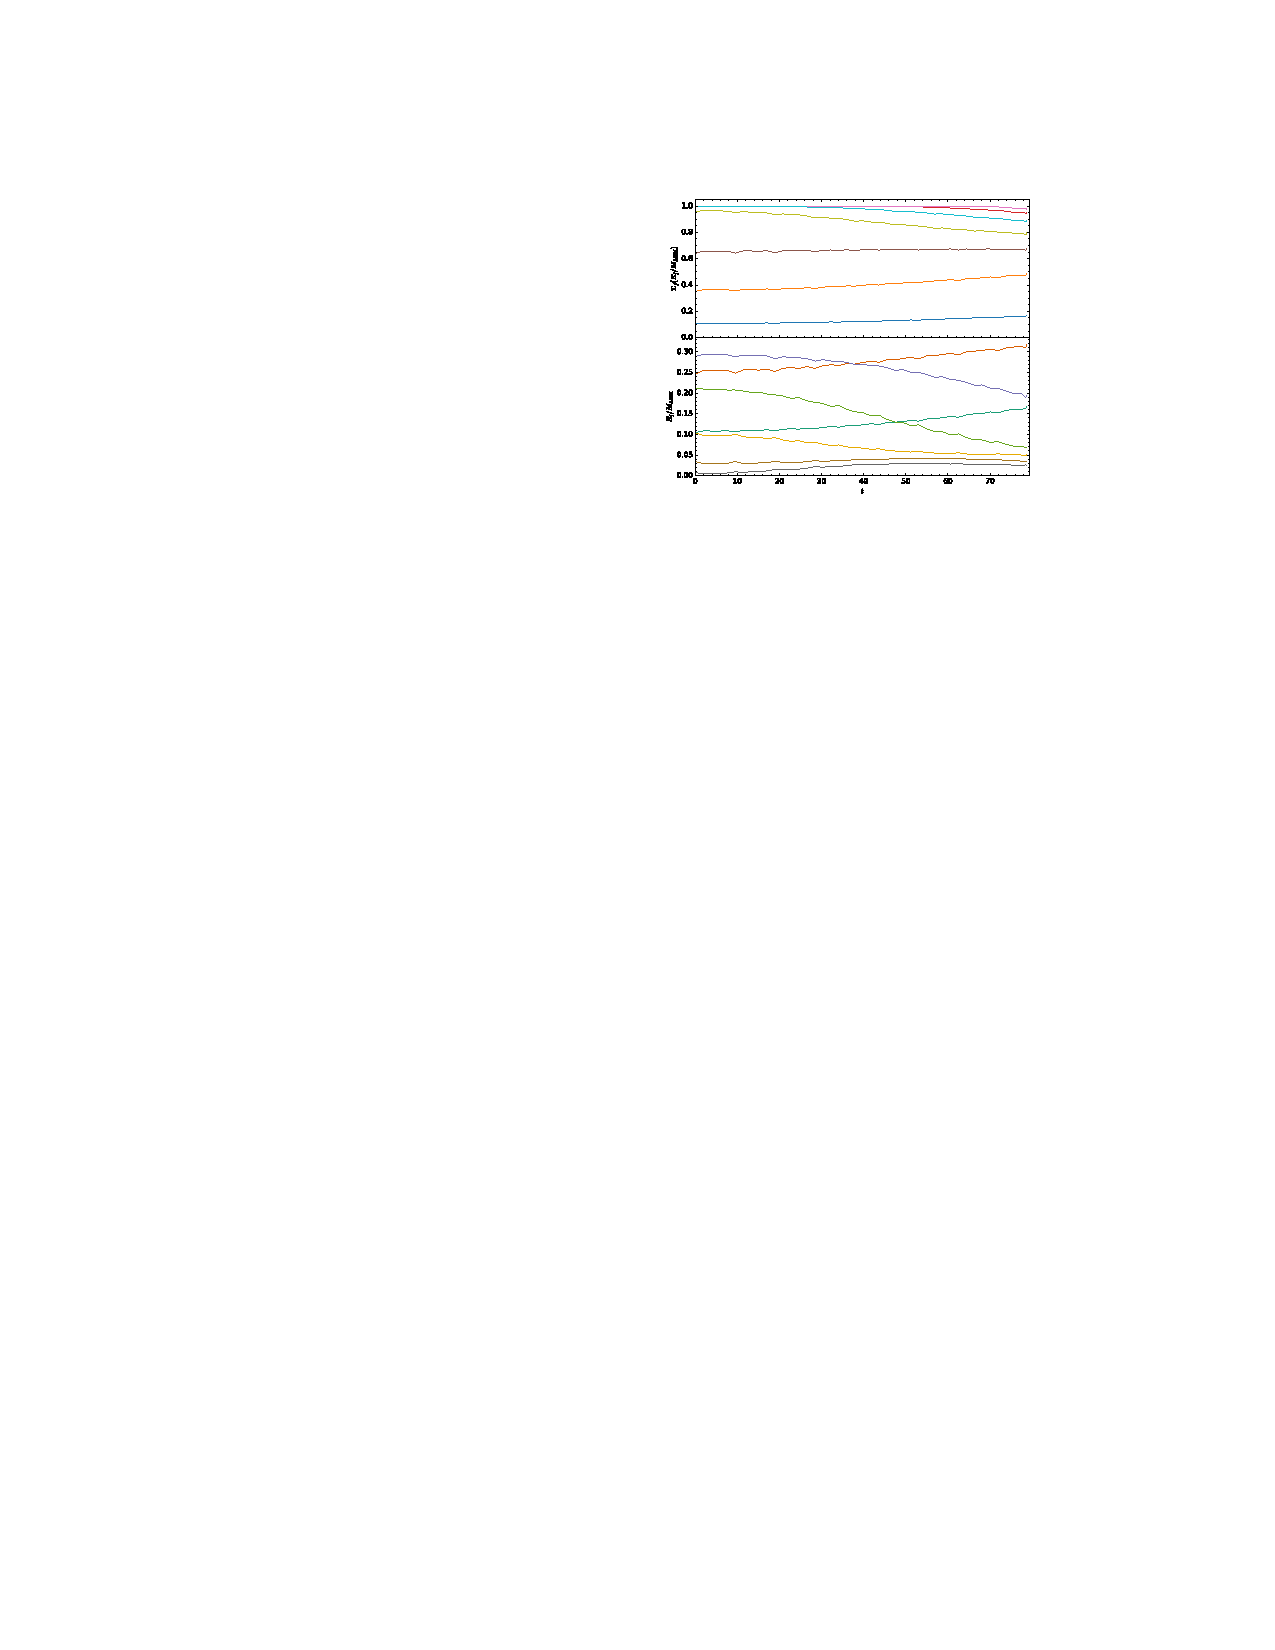
\includegraphics[width=\textwidth]{Em0w025} \\ $\mu = 0$, $\sigma = 0.25$, $\epsilon=2.28$ \\ Unstable
      \end{figure}
  \end{columns}
}
  
%%%%%%%%%%%%%%%%%%%%%%%%%%%%%%%%%%%%%%%%%%%%%%
%%%%%%%%%%%%%%%%%%%%%%%%%%%%%%%%%%%%%%%%%%%%%%

\section{High-Temperature QP Solutions in AdS$_4$}

\subsection{The Two-Time Formalism (TTF)}
\frame{
  \frametitle{The Two-Time Formalism (TTF) I}
  \bi
  \its Perturbative description of massless scalar field collapse $\to$ expand $\phi(t,x)$, $A(t,x)$, $\delta(t,x)$ in powers of small amplitude, $\epsilon$
  \its Consider TTF in AdS$_4$
  \its $\mc O(\epsilon)$: solution in terms of eigenfunctions of AdS, $e_j(x)$
  \its Truncate series to $\jm$ 
  \its Solutions must be robust as $\jm \to \infty$
  \its Develop numerical techniques for extending $\jm \gtrsim 100$ \& quantify effects of truncation
  \ei

  \begin{align*}
  \phi_1 (t,x) = \sum^\infty_{j=0} A_j(t) \cos (\omega_j t + B_j(t)) \: e_j (x)
  \end{align*}
}

\frame
{
  \frametitle{The Two-Time Formalism (TTF) II}
  \bi
  \its Integer eigenvalues $\omega_j = (2j + d)$ $\to$ fully resonant spectrum
  \its $\mc O(\epsilon^2)$: backreaction on metric
  \its $\mc O(\epsilon^3)$: \alert{source terms} for resonant contributions $\to$ resummation techniques absorb remaining resonances into amplitude/phase\footnotemark
  \its Energy exchange between modes through slowly varying amplitude $A_j(\tau)$ and phase $B_j(\tau)$ to resist collapse\footnotemark
  \its Define slow time $\tau \equiv \epsilon^2 t$
  \ei
  \vspace{-0.1in}
  \begin{align*}
  - 2 \omega_l \frac{d A_l (\tau)}{d \tau} &= \stackrel{l \leq i + j}{\sum_{i \neq l} \sum_{j \neq l}} \alert{f_1} \left(A_i, A_j, A_{i+j-l}, B_i, B_j, B_{i+j-l} \right) \\
  -2 \omega_l A_l \frac{d B_l(\tau)}{d \tau} &= \stackrel{l \leq i + j}{\sum_{i \neq l} \sum_{j \neq l}} \alert{f_2} \left(A_i, A_j, A_{i+j-l}, B_i, B_j, B_{i+j-l} \right)
  \end{align*}

  \footnotetext[7]{{\scr Craps {\it et al.} [1407.6273]}}
  \footnotetext[8]{{\scr Balasubramanian {\it et al.} [1403.6471]}}
}

%%%%%%%%%%%%%%%%%%%%%%%%%%%%%%%%%%%%%%%%%%%%%%

\subsection{Quasi-Periodic Solutions}
\frame
{
  \frametitle{Quasi-Periodic Solutions}
  \bi
  \its Quasi-periodic\footnotemark\ ansatz $A_j = \alpha_j e^{i \beta_j \tau}$ $\to$ TTF equations become time-independent when $\beta_j = \beta_0 + j(\beta_1 - \beta_0)$
  \its $\alpha_j > \alpha_{j+1} \: \forall \: j $
  \its Scaling symmetry (full {\bf and} TTF theory) $A(\tau) \to \epsilon A(\tau / \epsilon^2)$ allows for $\alpha_0 = 1$ $\to$ families of solutions in $\alpha_1$ 
  \its Origin of collapse time $t_H \approx a \epsilon^{-p} + b$ in nonlinear profiles
  \its Solve QP equation with Newton-Raphson $\to$ seed equation $\alpha_j \propto e^{-j}$ for low $\jm$
  \its $T_i$, $R_{ij}$, $S_{ijkl}$ calculated numerically
  \ei
  
   \begin{align*}
  2\omega_l \alpha_l \beta_l = T_l \alpha_l^3 + \sum_{i \neq l} R_{il} \alpha_i^2 \alpha_l + \stackrel{l \leq i + j}{\sum_{i \neq l} \sum_{j \neq l}} S_{i j (i+j-l)l} \alpha_i \alpha_j \alpha_{i+j-l}
  \end{align*}
  
  \footnotetext[9]{{\scr Green {\it et al.} [1507.08261]}}
}

\frame
{
  \frametitle{Quasi-Periodic Solutions}
  \bi
  \its TTF: conserved quantities\footnotemark\ $E$, $N$ $\to$ classify solutions by $T \equiv E/N$
  \its Solutions found for $3 \geq T \gtrsim 4.6$
  \its Able to extend existing solutions from $\jm \sim 100$ to $\jm = 500$
  \its Robust in $\jm \to \infty$ limit
  \ei
  
  \vspace{-0.1in}
  \begin{columns}
  \column{0.5\textwidth}
  \begin{figure}
  \centering
  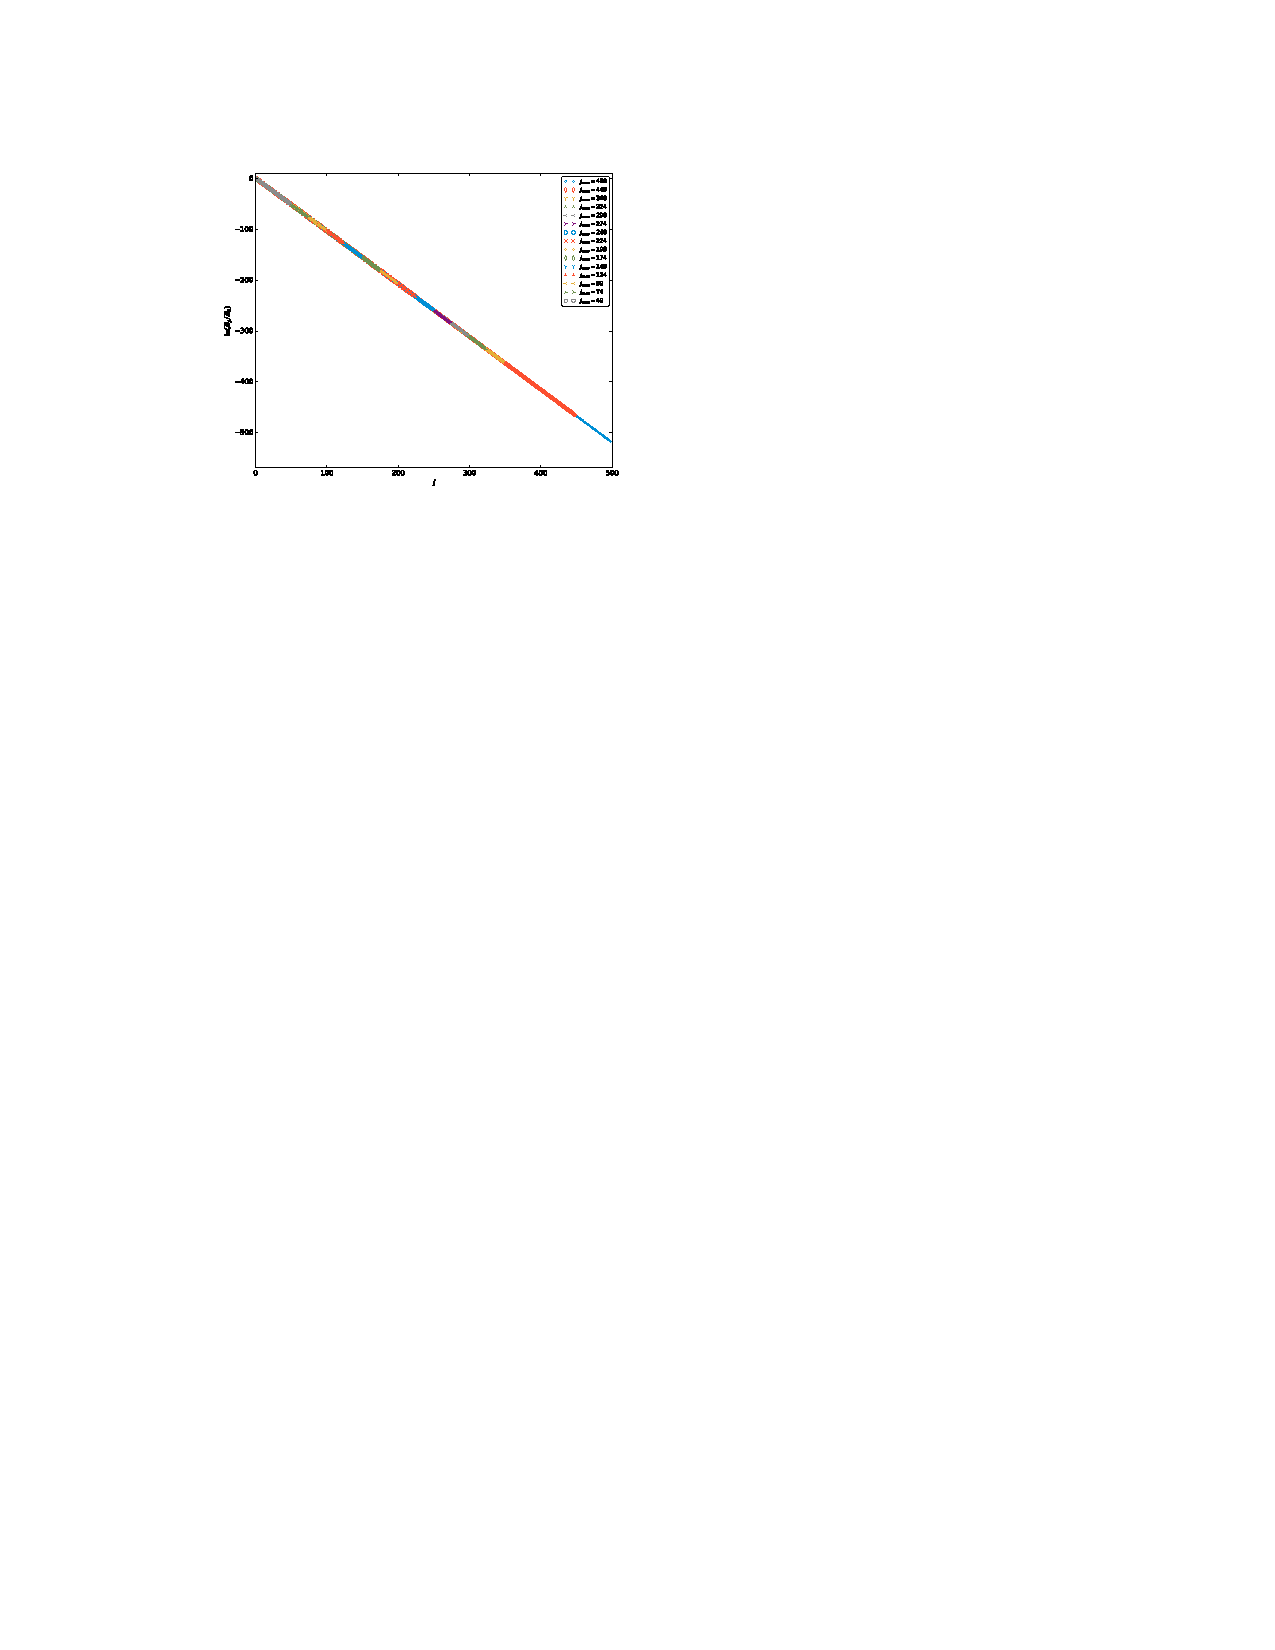
\includegraphics[scale=0.75]{largejmax} 
  \end{figure}
  \column{0.5\textwidth}
  \begin{figure}
  \centering
  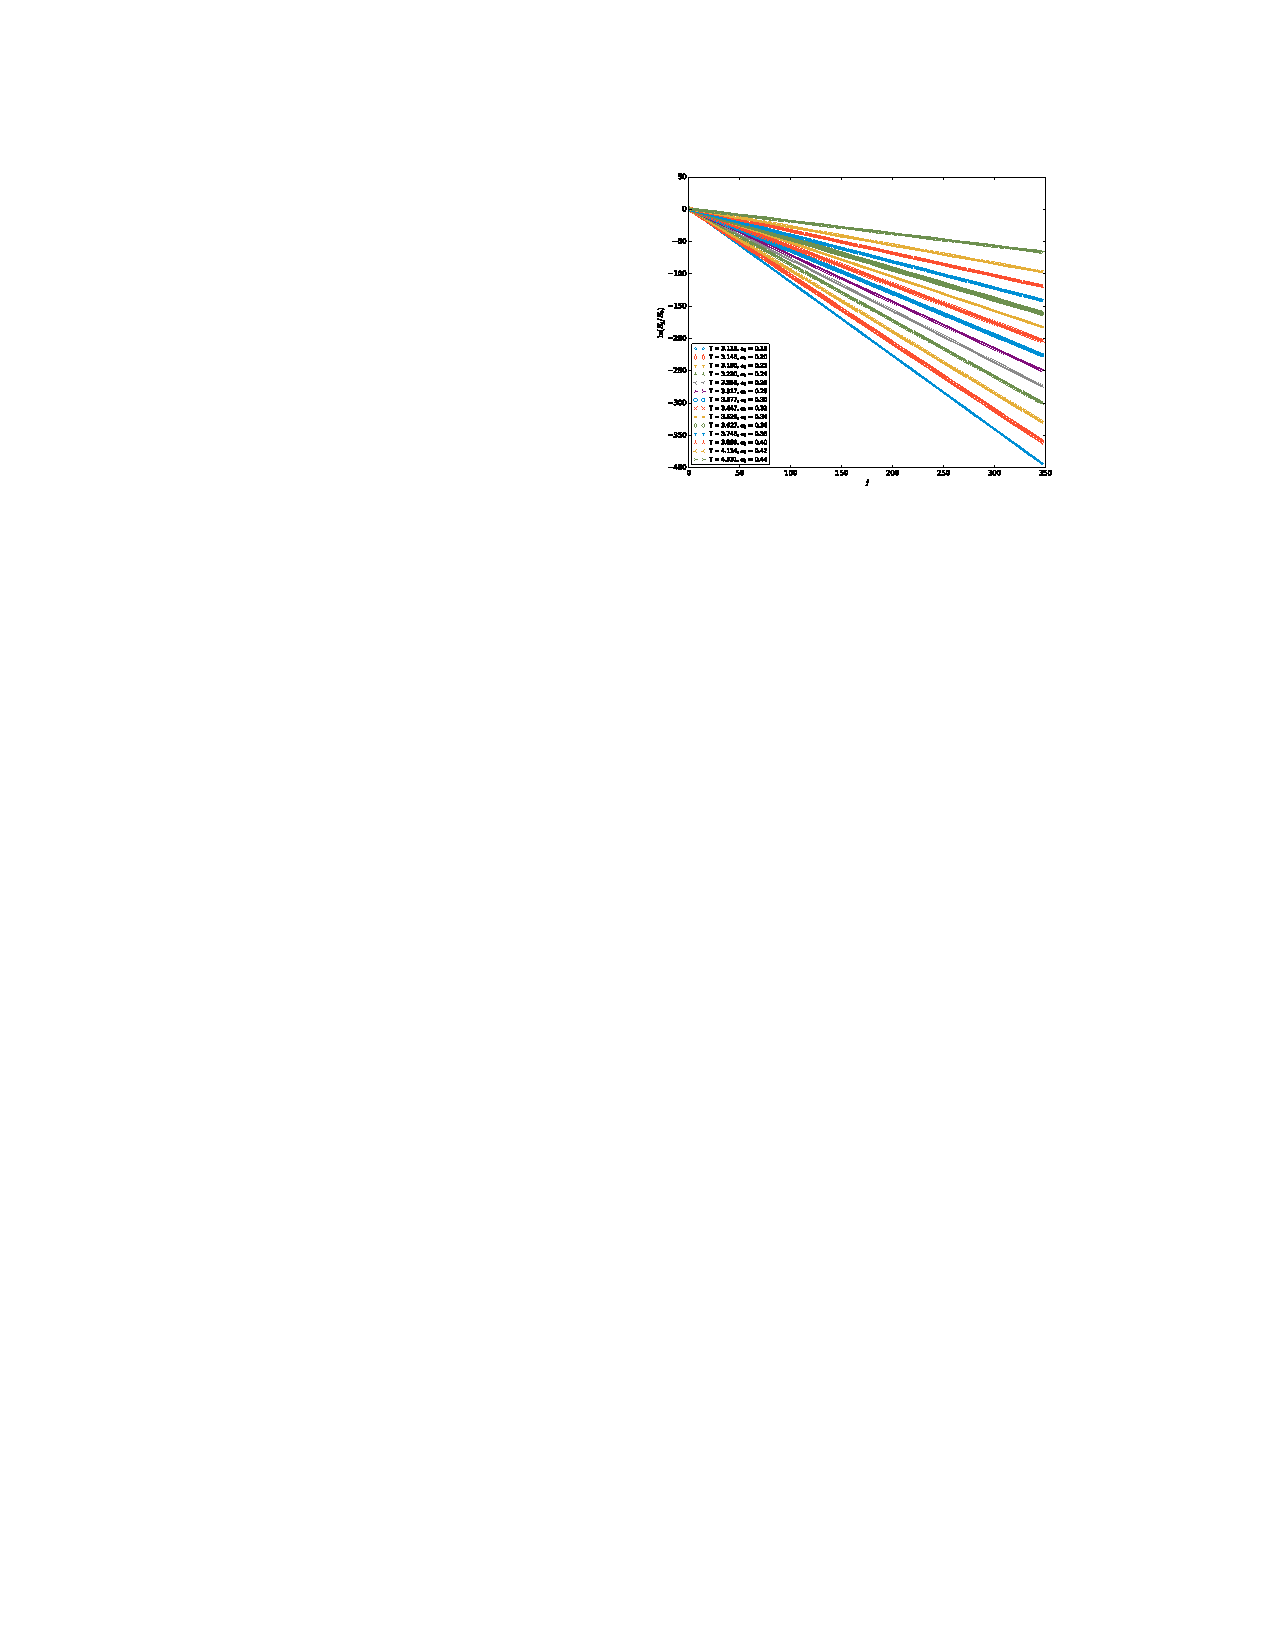
\includegraphics[scale=0.75]{families}
  \end{figure}
  \end{columns}
  \begin{center}
  {\scr BC, Deppe, \& Frey: In progress}
  \end{center}
  
  \vfill
  
  \footnotetext[10]{{\scr Craps {\it et al.} [1412.3249]}}
}

\frame
{
  \frametitle{High-Temperature Solutions}
  \bi
  \its Perturb by $\delta E$ $\to$ new solutions have energy $E + \delta E$, N, and $T + \delta T$
  \its Repeat process to $T_{max} = (2\jm + d)$
  \its Vary projection frequency back to solution plane $\to$ threshold \\ temperature $T_{th}$
  \ei
  
  \vspace{-0.15in}
  \begin{columns}
  \column{0.5\textwidth}
  \begin{figure}
  \centering
  \hspace{0.1in}
  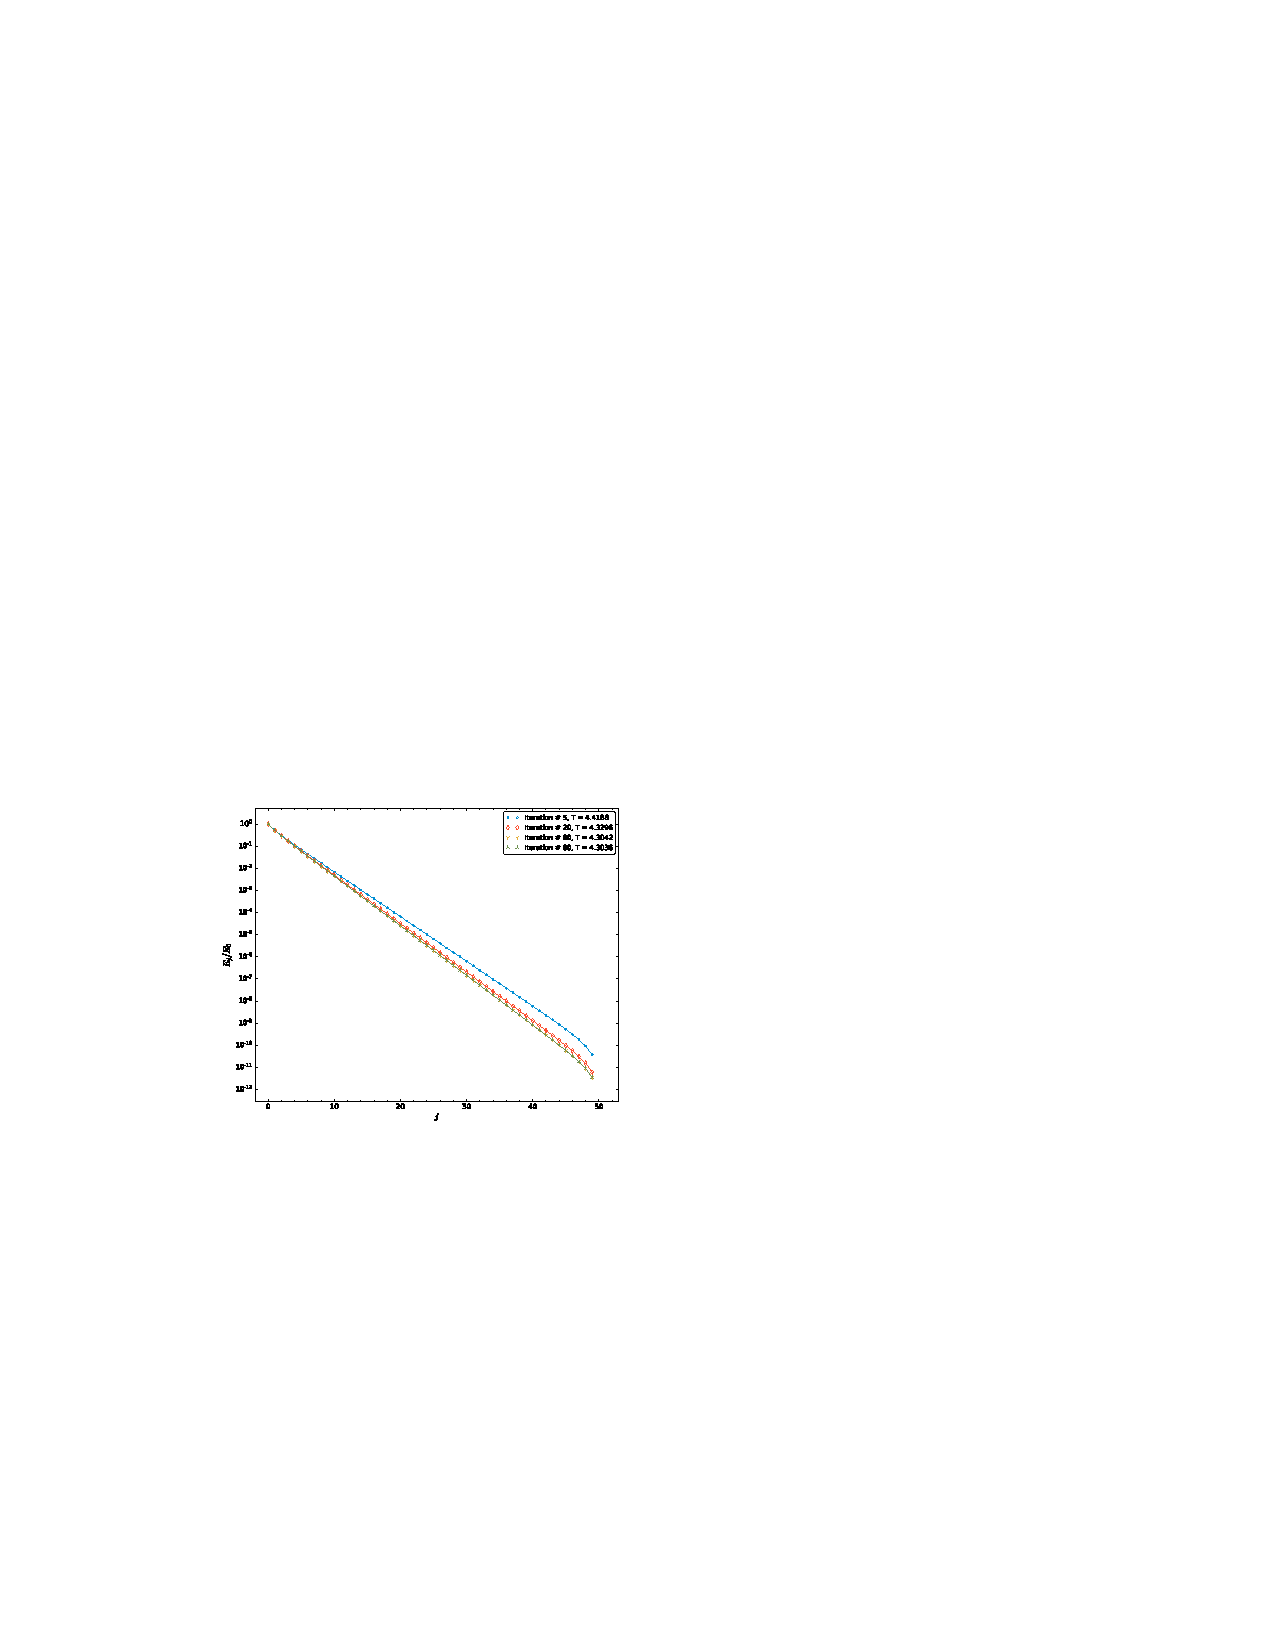
\includegraphics[scale=0.75]{reop5}
  \end{figure}
  \column{0.5\textwidth}
  \begin{figure}
  \centering
  \hspace{-0.1in}
  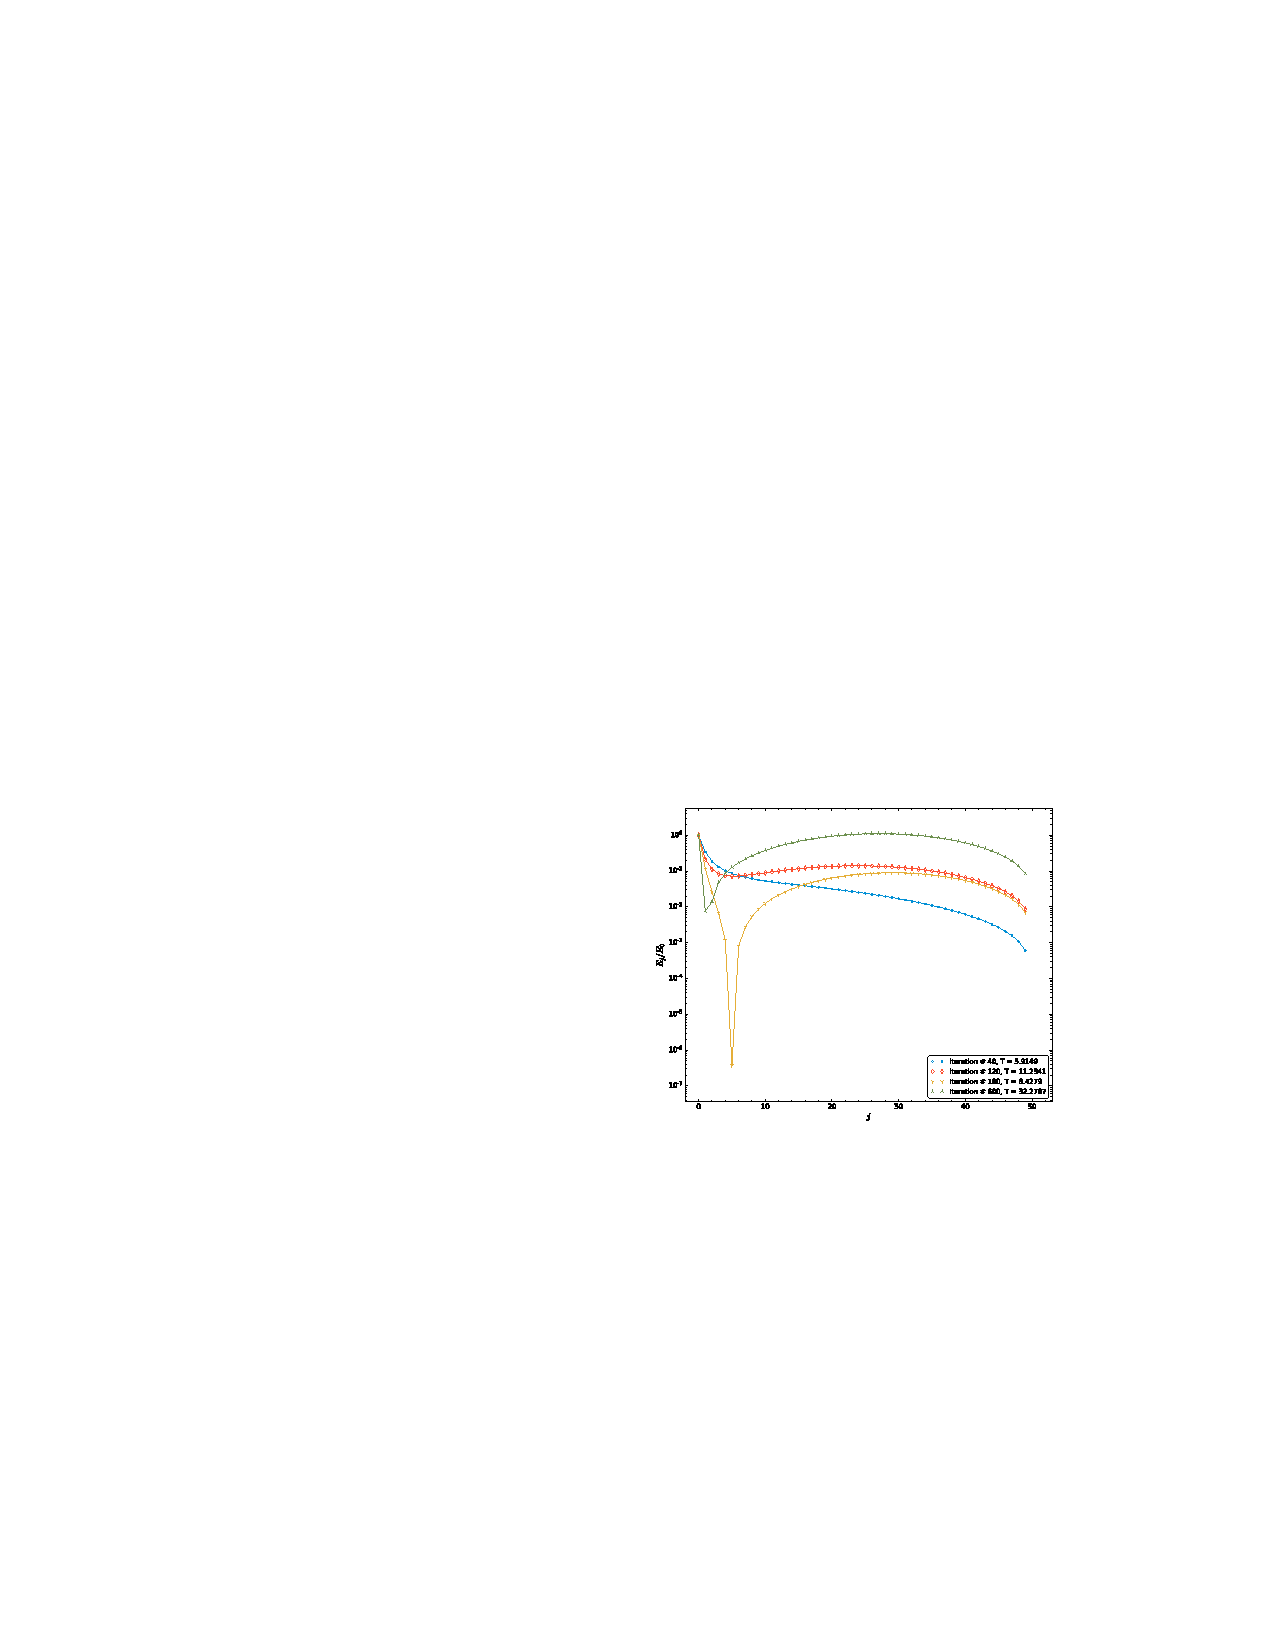
\includegraphics[scale=0.75]{reop20}
  \end{figure}
  \end{columns}
  \begin{center}
  \vspace{-0.12in}
  {\scr Cownden, Deppe, \& Frey: In progress}
  \end{center}
  \vspace{-0.1in}
  \bi
  \its If $T > T_{th}$, \alert{not robust} in $\jm \to \infty$
  \its $T_{th} << T_{max}$
  \ei
%\marginnote{\pdfcomment[icon=note]{(L) reop 5}}
%\marginnote{\pdfcomment[icon=note]{(R) reop 20}}
}

\frame[shrink]
{
  \frametitle{Evolving TTF Solutions}
  \bi
  \its Evolution of: \href{run:./Qpa4_40e-01j100eps0_01.mp4}{\beamerbutton{low-temperature QP $\triangleright$}} \: \href{run:./HighTa1_779e-01j100T2_0000e+01eps0_1.mp4}{\beamerbutton{high-temperature QP $\triangleright$}}
  \uncover<2->{\its Energy in $j=0,1,2,3$ modes (purple, green, blue, orange)}
  \uncover<3->{\its Residuals of QP equation}
  \ei
  \vspace{-0.2in}
  \uncover<1->{
  \begin{columns}
    \column{0.5\textwidth}
      \begin{figure}
      \centering
      \only<1>{
      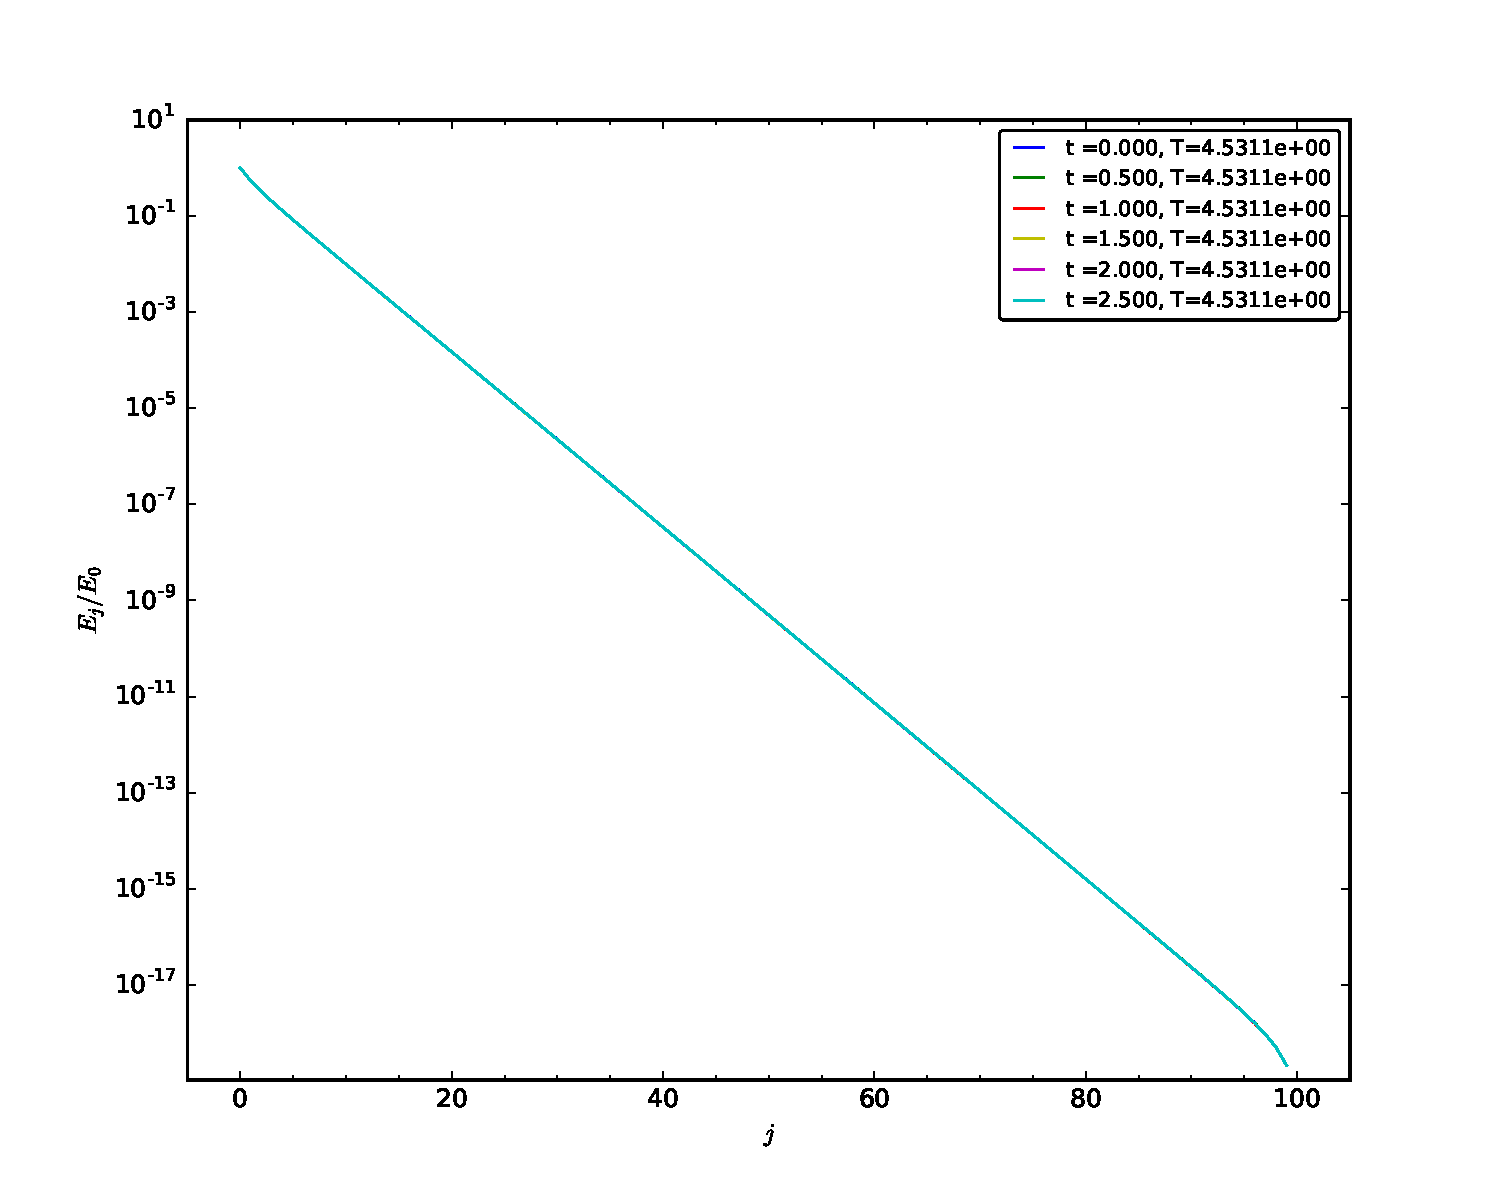
\includegraphics[width=\textwidth]{Qpa4_40e-01j100_specevo}
      }
       \only<2>{
      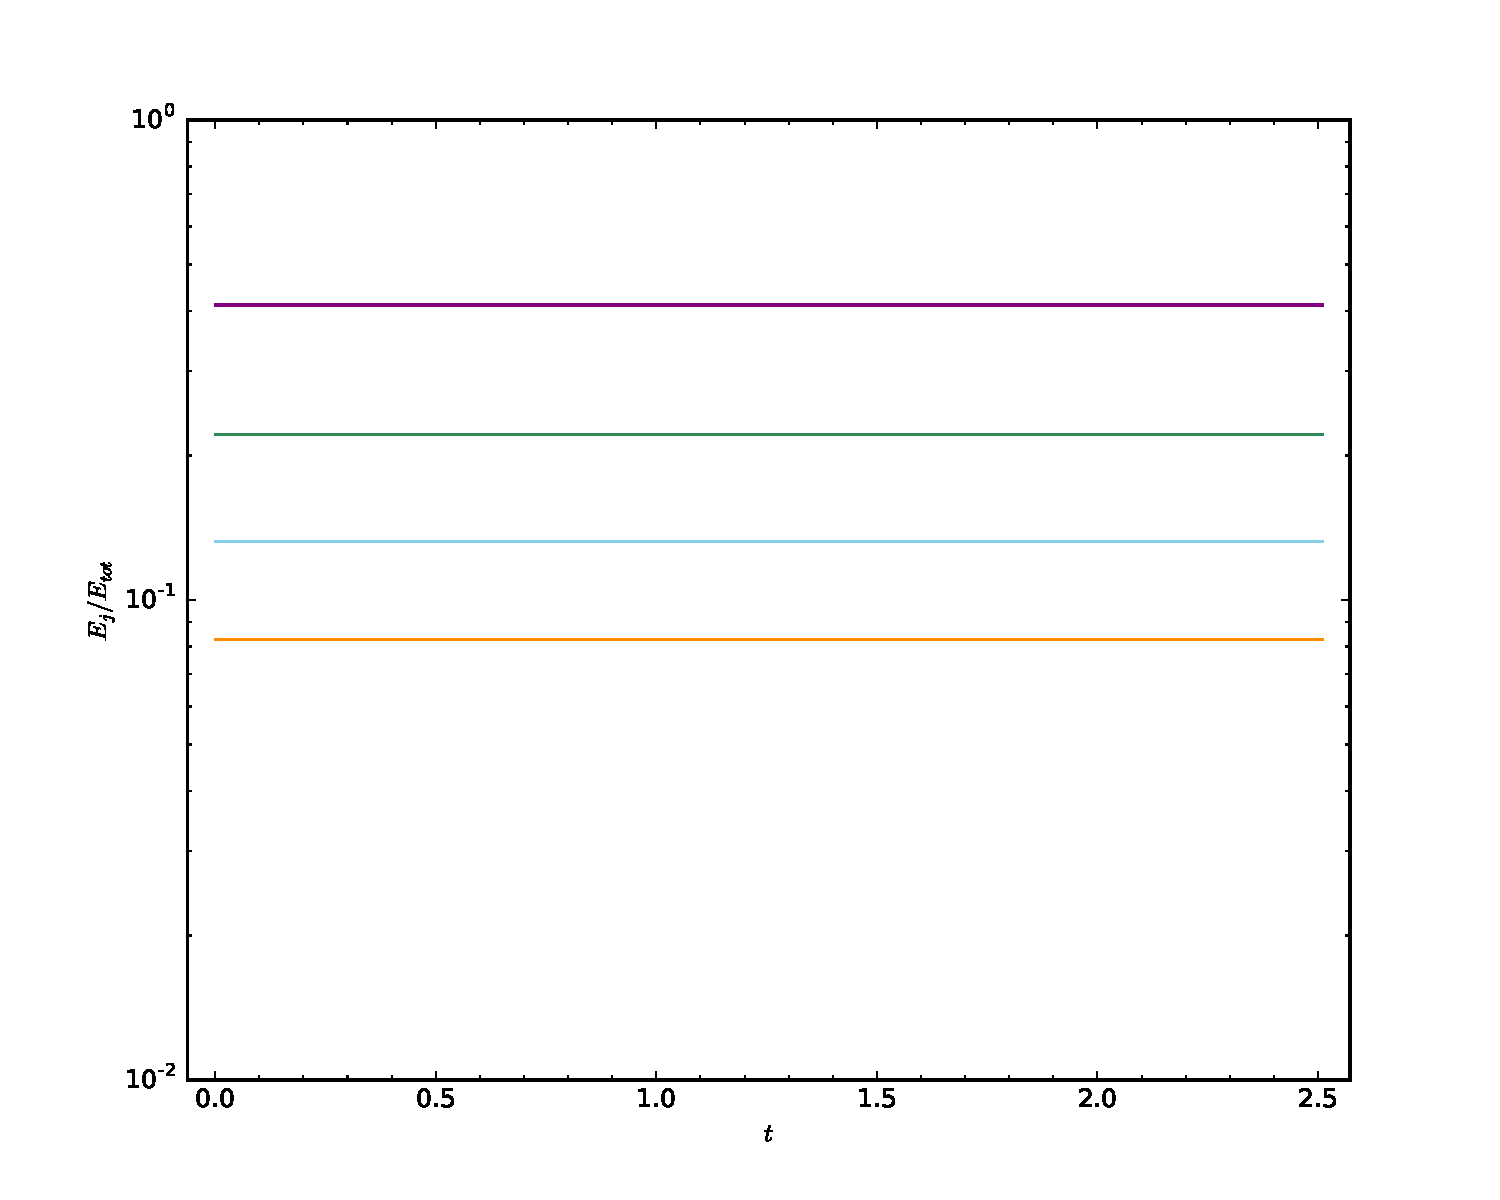
\includegraphics[width=\textwidth]{QPa2_00e-01_j100_lowjenergyevo}  
      }
      \only<3>{
      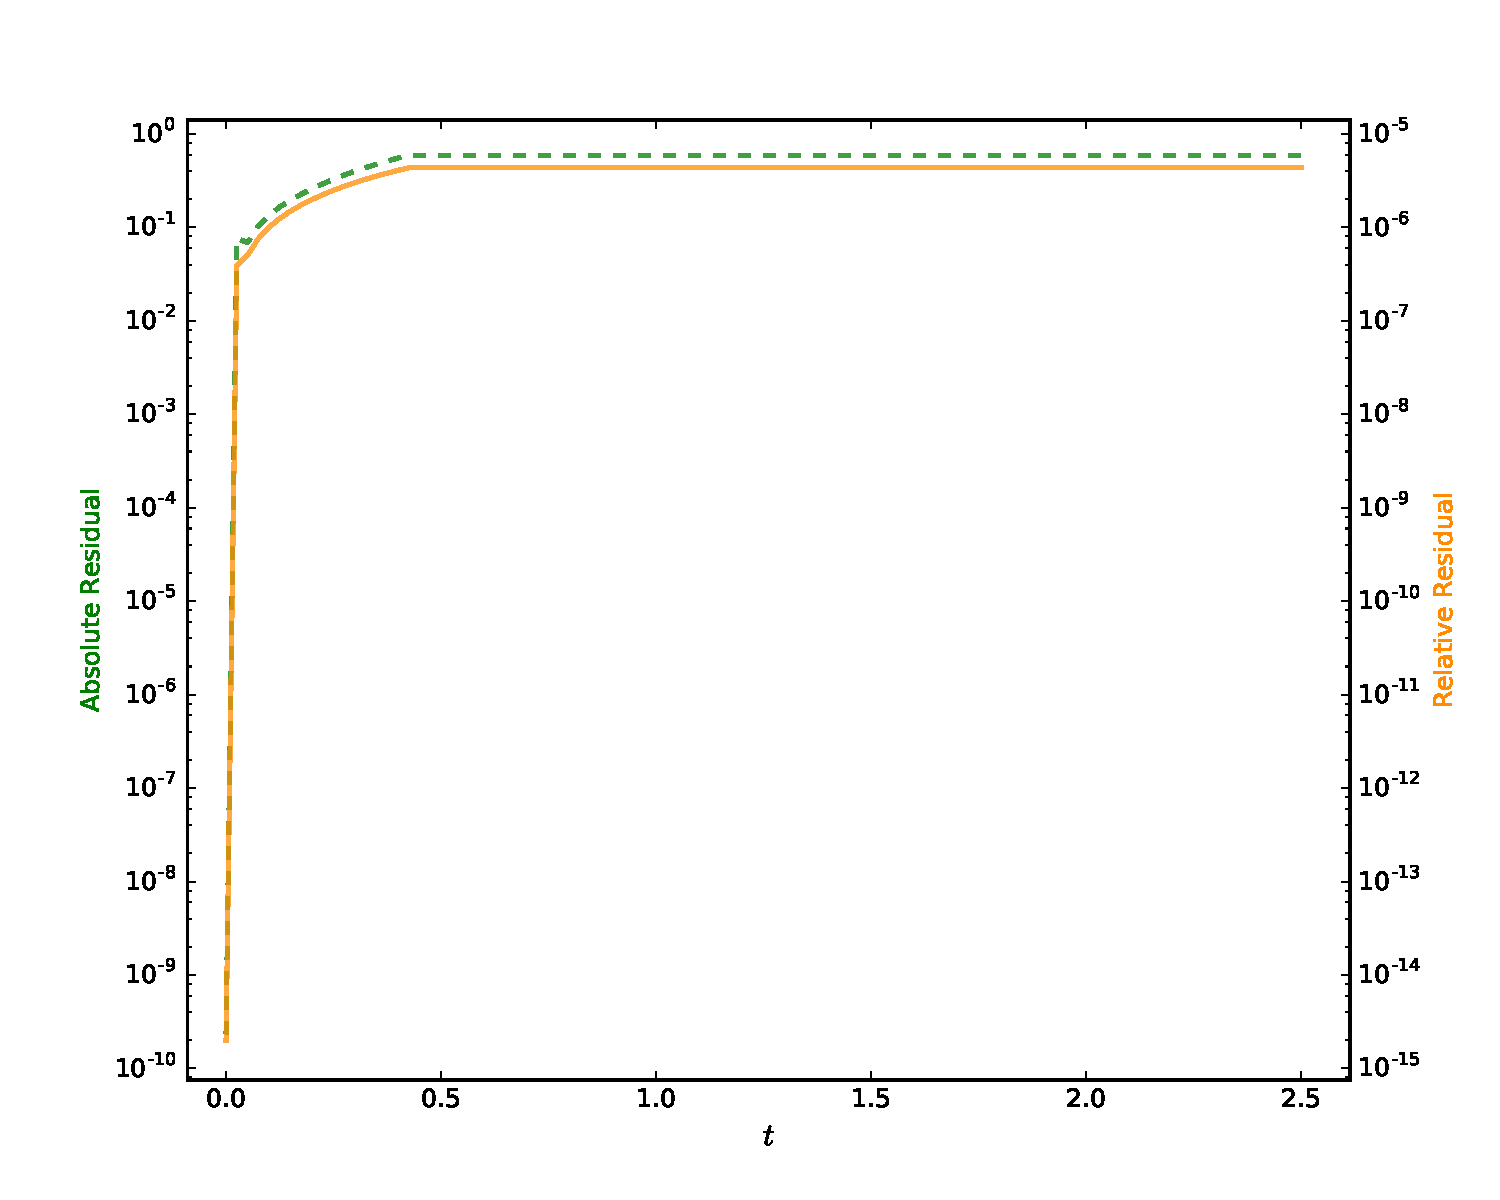
\includegraphics[width=\textwidth]{Qpa4_40e-01QPresids} 
      }
      \begin{center} Low-temperature \end{center}
      \end{figure}
    \column{0.5\textwidth}
      \begin{figure}
      \centering
      \only<1>{
      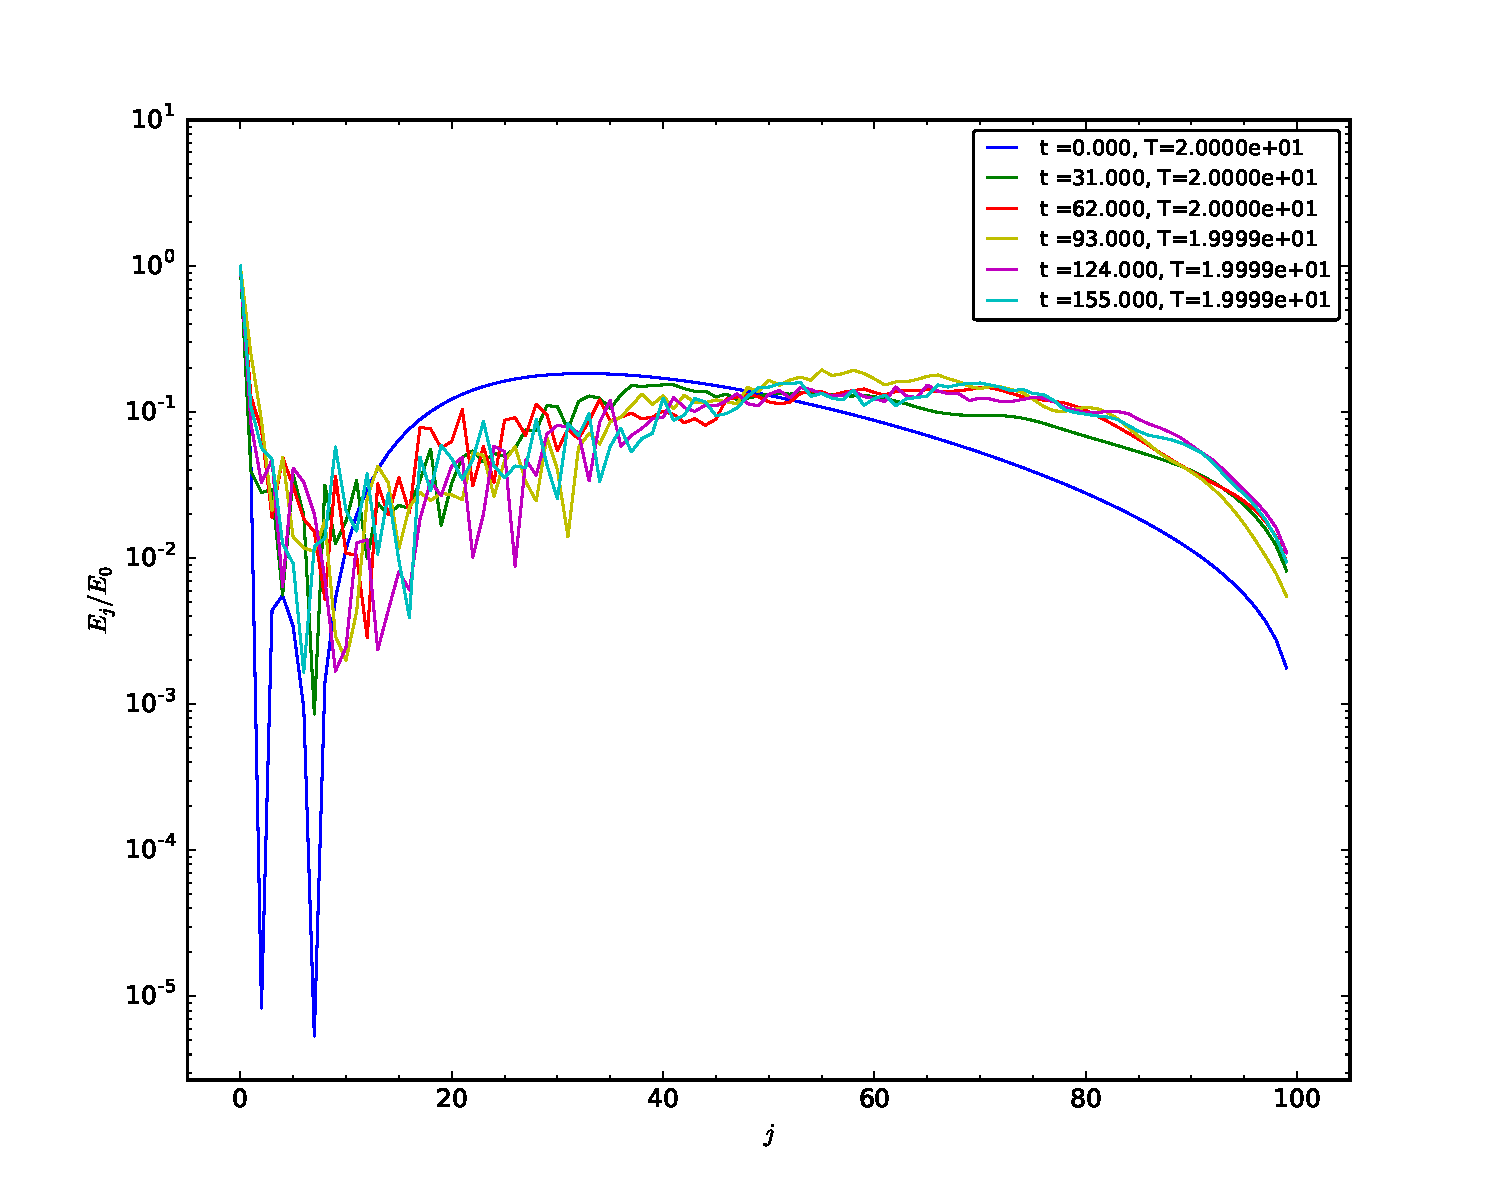
\includegraphics[width=\textwidth]{HighTa1_779e-01j100T2_0000e+01_specevo}
      }
      \only<2>{
      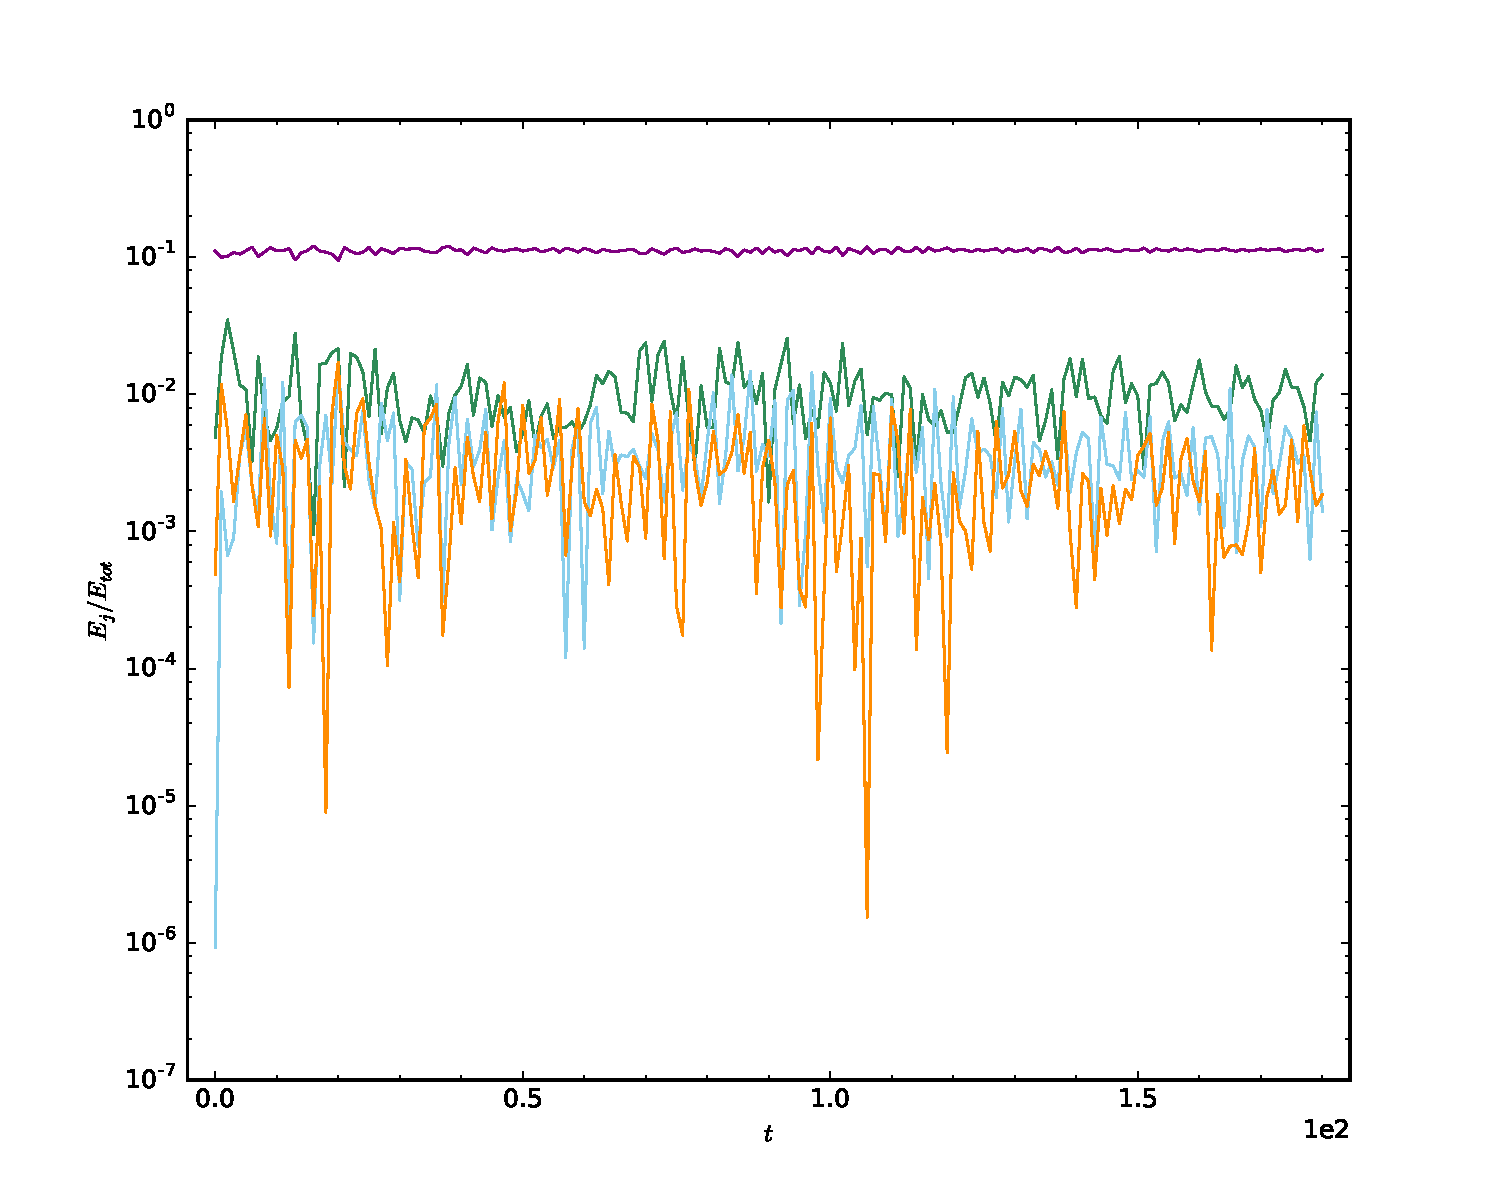
\includegraphics[width=\textwidth]{HighTa1_779e-01j100T2_0000e+01_lowjevo}
      }
      \only<3>{
      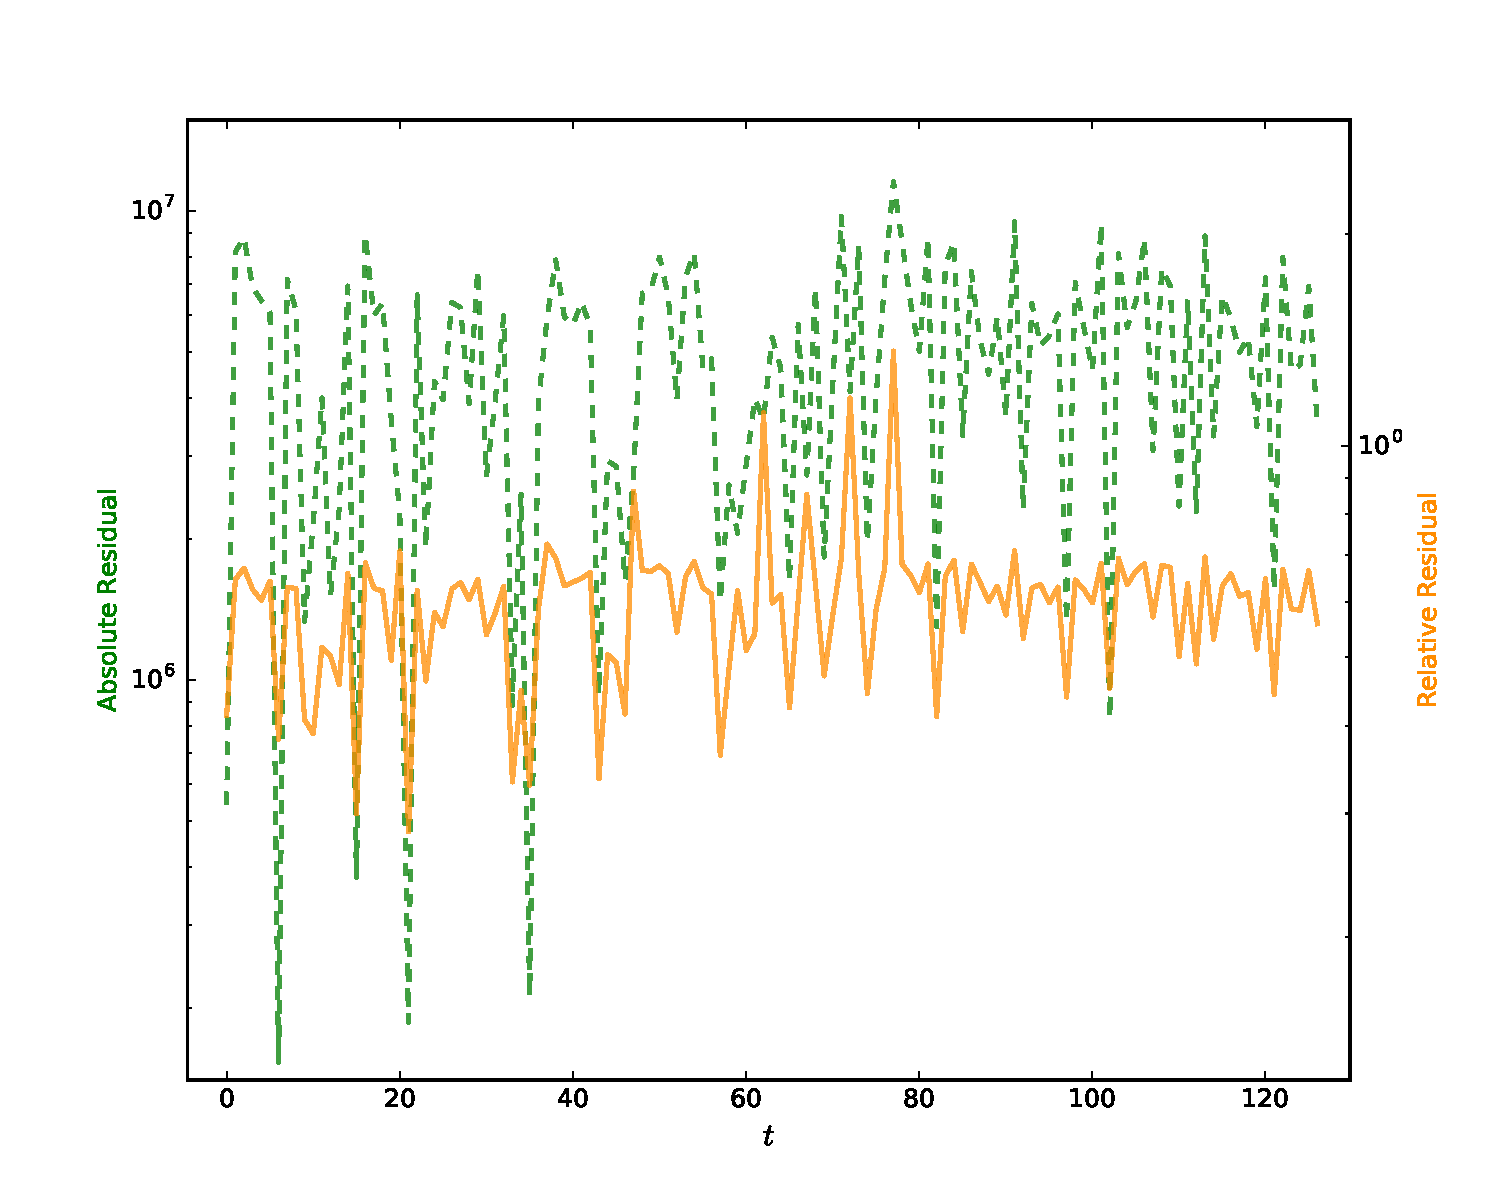
\includegraphics[width=\textwidth]{HighTresiduals} 
      } 
       \begin{center} High-temperature \end{center}
      \end{figure}
  \end{columns}
  }
}


%%%%%%%%%%%%%%%%%%%%%%%%%%%%%%%%%%%%%%%%%%%%%%

\subsection{Outstanding Questions}
\frame
{
  \frametitle{Outstanding Questions}
  \begin{columns}
  \column{0.45\textwidth}
    \bi
    \its Physical interpretation for $T_{th}$?
    \its Is $| T_{QP} - T_{th}|$ a function of AdS parameters? What does this mean for boundary CFT?
    \its Compare perturbative evolution to full numerical $\to$ establish absolute timescale for approximation
    \its Use high-temperature QP solutions as initial data in nonlinear evolution $\to$ metastable/irregular? What is mechanism of collapse?
    \ei
  \column{0.55\textwidth}
    \begin{figure}
      \centering
      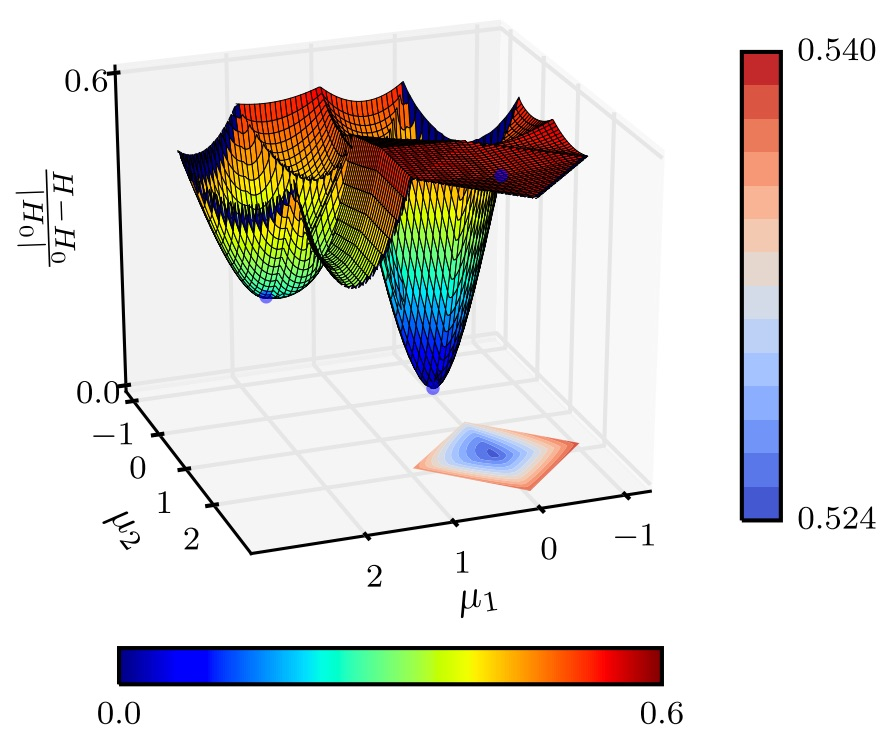
\includegraphics[width=\textwidth]{Green_hamiltonian} \\ {\scr Green {\it et al.} [1507.08261]}
    \end{figure}
  \end{columns}
}

%%%%%%%%%%%%%%%%%%%%%%%%%%%%%%%%%%%%%%%%%%%%%%
%%%%%%%%%%%%%%%%%%%%%%%%%%%%%%%%%%%%%%%%%%%%%%

\section{Examining Instabilities Due to Driven Scalars in AdS [arXiv:1912.07143]}
\subsection{Time-dependent Boundary Conditions}
\frame
{
  \frametitle{Time-dependent Boundary Conditions}
}

%%%%%%%%%%%%%%%%%%%%%%%%%%%%%%%%%%%%%%%%%%%%%%

\subsection{Resonant Contributions}
\frame
{
  \frametitle{Resonant Contributions}
}

%%%%%%%%%%%%%%%%%%%%%%%%%%%%%%%%%%%%%%%%%%%%%%

\subsection{Special Values of Non-normalizable Frequencies}
\frame
{
  \frametitle{Special Values of Non-normalizable Frequencies}
}

%%%%%%%%%%%%%%%%%%%%%%%%%%%%%%%%%%%%%%%%%%%%%%
%%%%%%%%%%%%%%%%%%%%%%%%%%%%%%%%%%%%%%%%%%%%%%

{
  \AtBeginSection[]{}
\section{Conclusions}
\frame
{
   \frametitle{Conclusions}
   \bi
   \its Collapse of scalar field in AdS $\Leftrightarrow$ thermalization of dual CFT
   \its {\bf Nonlinear theory:} ``islands of stability'', metastable \& irregular phases, chaotic behaviour from self-interaction
   \its Weakly turbulent energy cascade to short length scales $\to$ TTF for inverse cascades 
   \its {\bf Perturbative theory:} QP solutions robust in $j_{max} \to \infty$, high-T solutions are not; space of stable solutions is restricted by $T_{th}$
   \its {\bf Next steps}
     \begin{itemize}
     \its Physical interpretation of $T_{th}$ 
     \its Ways to construct robust QP solutions with $T > T_{th}$
     \end{itemize}
   \its {\bf Future:} develop theory for \underline{\emph{massive}} TTF $\to$ less symmetry in equations $\therefore$ fewer cancelations of resonant terms; TTF in AdS$_5$; time-dependent boundary conditions
    \ei
}
\section*{}
\frame[noframenumbering]
{
   \frametitle{Thanks}
   \begin{itemize}
   \its Supervisor: Andrew Frey (University of Winnipeg)
   \its PhD Committee: (),  (), (),  ()
   \its Co-authors: Nils Deppe (Cornell), Brayden Yarish (junior collaborator)
   \its University of Winnipeg and University of Manitoba
   \end{itemize}
}

\frame[noframenumbering]
{
  \frametitle{References}
  \bi
  \its M. Choptuik, \emph{Universality and scaling in gravitational collapse of a massless scalar field}, Phys. Rev. Lett. 70 (1993) 9-12. 
  \its P. Bizo\'n and A. Rostworowski, \emph{On weakly turbulent instability of anti-de Sitter space}, Phys. Rev. Lett. 107 (2011) 031102, [1104.3702]. 
  \its N. Deppe and A. R. Frey, \emph{Classes of Stable Initial Data for Massless and Massive Scalars in Anti-de Sitter Spacetime}, JHEP 12 (2015) 004, [1508.02709]. 
  \its J. M. Maldacena, \emph{The Large N limit of superconformal field theories and supergravity}, Int. J. Theor. Phys. 38 (1999) 1113, [hep-th/9711200]. 
  \its R. Brito, V. Cardoso, and J. V. Rocha, \emph{Interacting shells in AdS spacetime and chaos}, Phys. Rev. D94 (2016), no. 2 024003, [1602.03535]. 
  \its N. Deppe, A. Kolly, A. R. Frey, and G. Kunstatter, \emph{Black Hole Formation in AdS Einstein-Gauss-Bonnet Gravity}, J. High Energ. Phys. (2016) 2016: 87, [1608.05402].
  \its B. Craps, O. Evnin, and J. Vanhoof, \emph{Renormalization group, secular term resummation and AdS (in)stability}, JHEP 10 (2014) 048, [1407.6273].
   \ei
}

\frame[noframenumbering]
{
  \frametitle{References}
  \bi
  \its V. Balasubramanian, A. Buchel, S. R. Green, L. Lehner, and S. L. Liebling, \emph{Holographic Thermalization, Stability of Anti-de Sitter Space, and the Fermi-Pasta-Ulam Paradox}, Phys. Rev. Lett. 113 (2014) 071601, [1403.6471].
  \its S. R. Green, A. Maillard, L. Lehner, and S. L. Liebling, \emph{Islands of stability and recurrence times in AdS}, Phys. Rev. D92 (2015) 084001, [1507.08261].
  \its B. Craps, O. Evnin, and J. Vanhhof, \emph{Renormalization, averaging, conservation laws and AdS (in)stability}, J. High Energ. Phys. 1501 (2015) 108, [1412.3249].
  \ei
}
}

\end{document}

%%%%%%%%%%%%%%%%%%%%%%%%%%%%%%%%%%%%%%%%%%%%%%
%%%%%%%%%%%%%%%%%%%%%%%%%%%%%%%%%%%%%%%%%%%%%%


